%% ------------------------------------------------------------------- %%
%% ------------------------------------------------------------------- %%
%% ------------------------------------------------------------------- %%
%% ------------------------------------------------------------------- %%
\chapter{Marco Conceptual}
\label{cap:marcoteorico}

\lhead{\emph{Marco Conceptual}} 

El proyecto pertenece al área de Bioinformática y específicamente a la Inmunoinformática, en este contexto el marco teórico detalla conceptos de Biología Molecular (ADN, ARN y proteínas), Inmunología y Ciencias de la Computación. 

\section{Bioinformática}

En esta sección, describiremos los principales conceptos referentes a Bioinformática que serán considerados en la propuesta de la tesis.

\subsection{Bioinformática}

Según \cite{luscombe2001bioinformatics}, la Bioinformática involucra la tecnología que utiliza las computadoras para el almacenamiento, manipulación y distribución de información relacionada a la Biología Molecular como DNA, RNA y proteínas. También podemos considerar que la Bioinformática se enfoca al análisis de secuencias, estructuras y funciones de los genes y proteínas. Adicionalmente, algunos autores como \cite{xiong2006essential} consideran a la Biología Molecular Computacional como un sinónimo a la Bioinformática.


\subsection{DNA, RNA y Proteínas}

\textit{Deoxyribonucleic Acid} (DNA) es una molécula dentro de las células que contiene información genética responsable del desarrollo y función del organismo \citep{NCIdictionary2022}. Gran parte del DNA se sitúa dentro del núcleo de las células (en organismos Eucariontes). Por ejemplo en la Figura \ref{img:dnalocation}, vemos como el DNA, forma parte de los cromosomas y estos a su vez están en el núcleo. Luego, podemos notar, que los genes representan segmentos del DNA. Finalmente, en la Figura \ref{img:dnalocation}, notamos las bases nitrogenadas que componen el DNA: \textit{Guanine}, \textit{Cytosine}, \textit{Adenine} y \textit{Thymine}; normalmente, estas bases serán representadas por las letras: G, C, A, T respectivamente.

\begin{figure}[H]
	\centering
	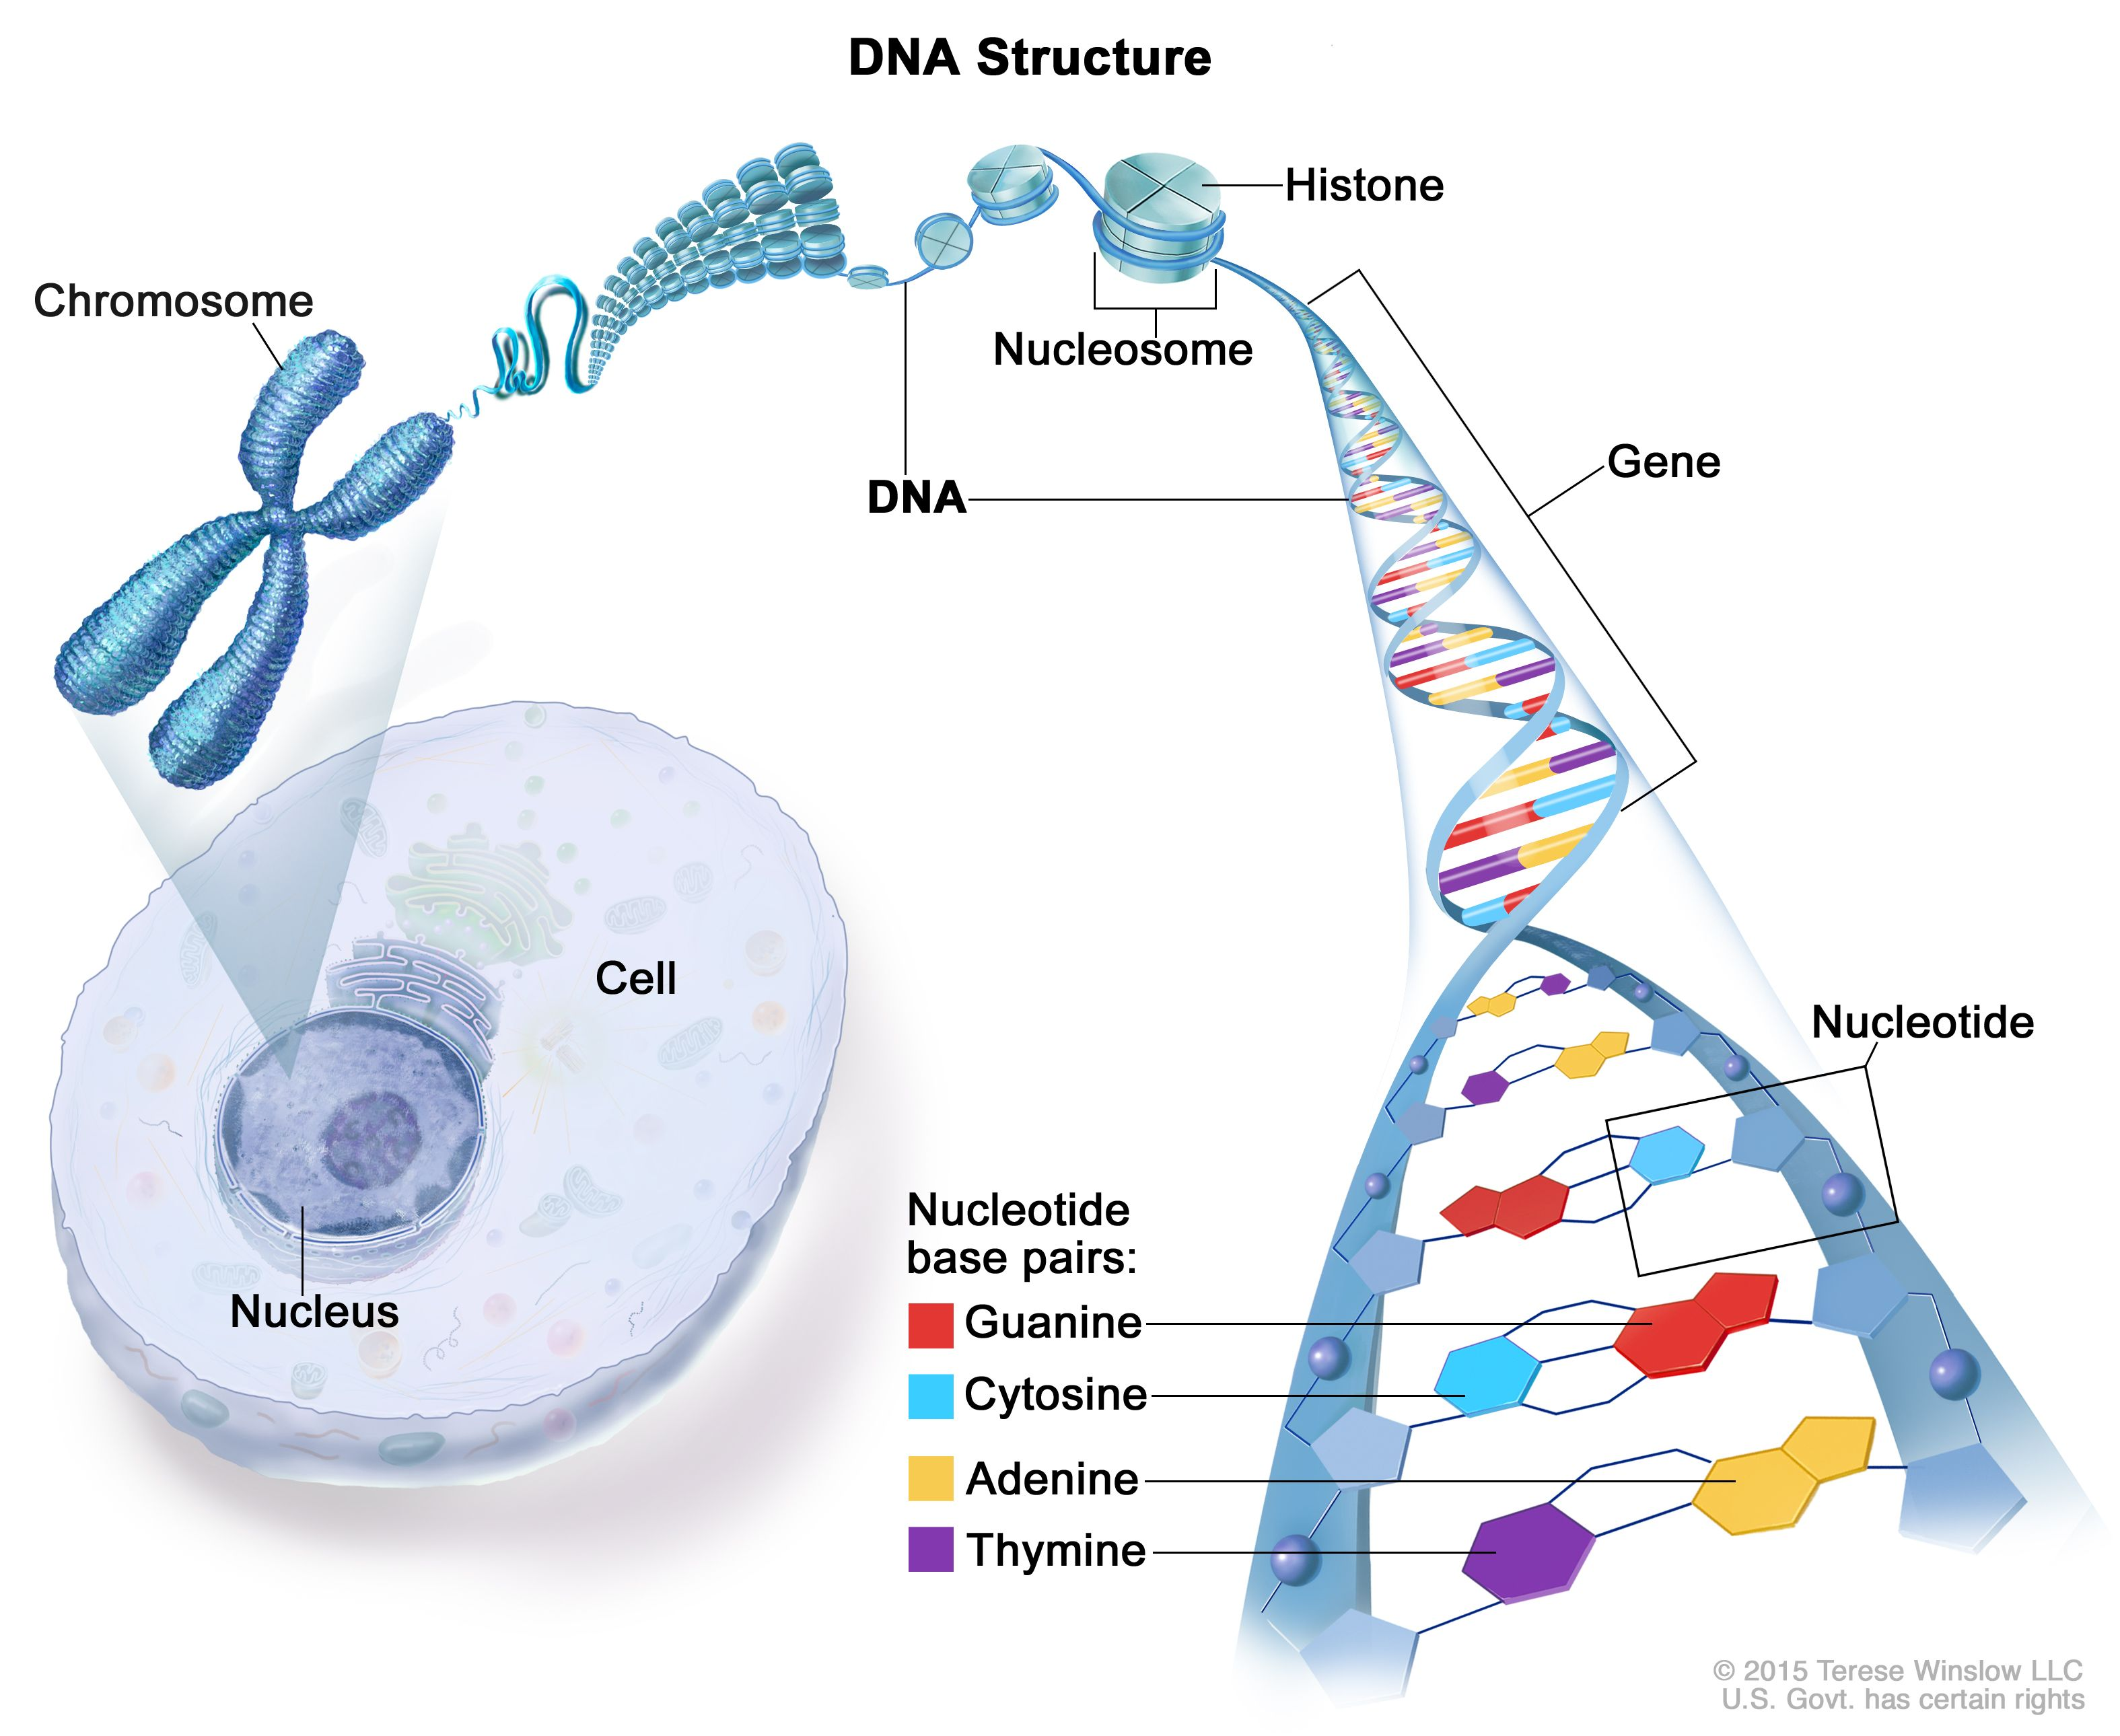
\includegraphics[width=0.8\textwidth]{../img/neoantigen/dna}
	\caption{Localización y estructura del DNA. Fuente:  \cite{NCIdictionary2022}.}	
	\label{img:dnalocation}
\end{figure}

Durante el ciclo de vida de la célula, ocurre un proceso llamado Transcripción (ver Figura \ref{img:trans}), en este proceso se generan cadenas de \textit{Ribonucleic Acid} (RNA) a partir de la cadena de DNA \citep{NCIdictionary2022}.  Durante este proceso la base nitrogenada \textit{Thymine} (T) es reemplazada por \textit{Uracil} (U). El proceso mencionado, ocurre dentro del núcleo de la célula y en esta etapa el RNA es llamado \textit{messenger RNA} (mRNA). Una vez el mRNA sale del núcleo, es transportado por \textit{transfer RNA} (tRNA) hacia los Ribosomas (ver Figura \ref{img:trans}). En está, última etapa ocurre la Traducción, cada grupo de tres bases nitrogenadas (codones) se convierten en un aminoácido diferente, luego estos aminoácidos forman cadenas polipeptídicas y estas a su vez forman las proteínas; normalmente, cada gen genera una proteína \citep{xiong2006essential, NCIdictionary2022}.



\begin{figure}[]
	\centering
	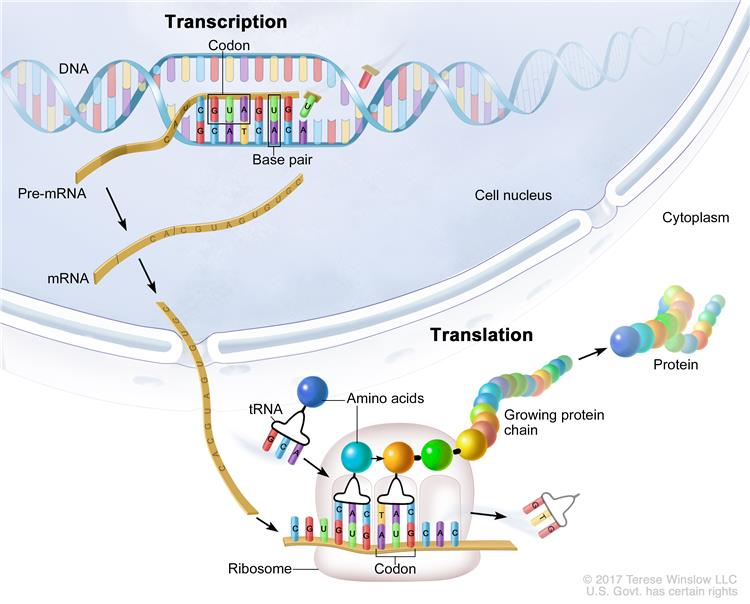
\includegraphics[width=0.8\textwidth]{../img/neoantigen/trans}
	\caption{Transcripción y traducción. Fuente:  \cite{nci2020}.}	
	\label{img:trans}
\end{figure}

Durante el proceso de Traducción, puede ocurrir un fenómeno llamado \textit{Alternative Splicing}. Por ejemplo , en la Figura \ref{img:alt}, notamos como un gen puede generar tres proteínas distintas, cada una con funciones distintas. Este fenómenos, complica bastante el análisis de DNA.


\begin{figure}[]
	\centering
	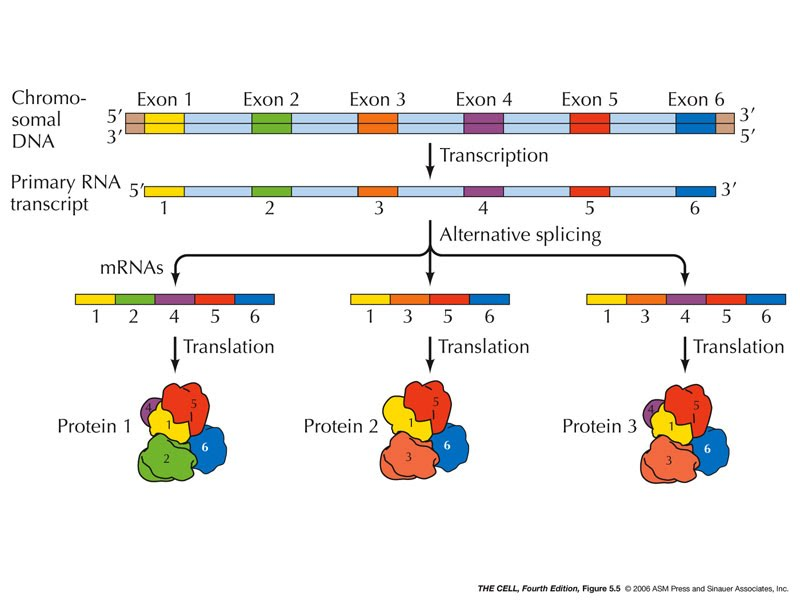
\includegraphics[width=0.9\textwidth]{../img/neoantigen/alt}
	\caption{\textit{Alternative Splicing}. Fuente:  \cite{nci2020}.}	
	\label{img:alt}
\end{figure}


\subsection{Mutaciones}

Las mutaciones también llamadas variaciones, representan cualquier cambio en la secuencia de DNA, estos pueden ocurrir durante la división celular o por la exposición a agentes químicos o radioactivos. Estas mutaciones pueden ser beneficiosas, dañinas (cuando afectan la generación de proteínas) o no tener algún efecto  \citep{NCIdictionary2022}. Varios tipos de Cáncer son ocasionados por estas mutaciones \citep{borden2022cancer, chen2021challenges, de2020neoantigen}. 

Según el tipo de célula afectada, tenemos: mutaciones somáticas y mutaciones \textit{germline} (una mutación en estas células puede ser heredada a la descendencia) \citep{clancy2008genetic}.  Según \citep{xu2018review}, las variaciones genómicas pueden clasificarse en tres grupos: \textit{Single-Nucleotide Variant} (SNV), inserciones y eliminaciones (INDELS) y \textit{Structural Variation} (SV). Una mutación se considera SNV cuando las variaciones afectan a menos de 10 bases. 

En la Figura \ref{fig:SNV}, presentamos ejemplos de SNV. Por ejemplo, las sustituciones pueden afectar la generación de un aminoácido, pero las inserciones o eliminaciones pueden afectar en cadena la generación de varios aminoácidos, a este tipo de fenómeno se le conoce como \textit{frameshit mutation} \citep{xu2018review}.


\begin{figure}[h]
	\centering
	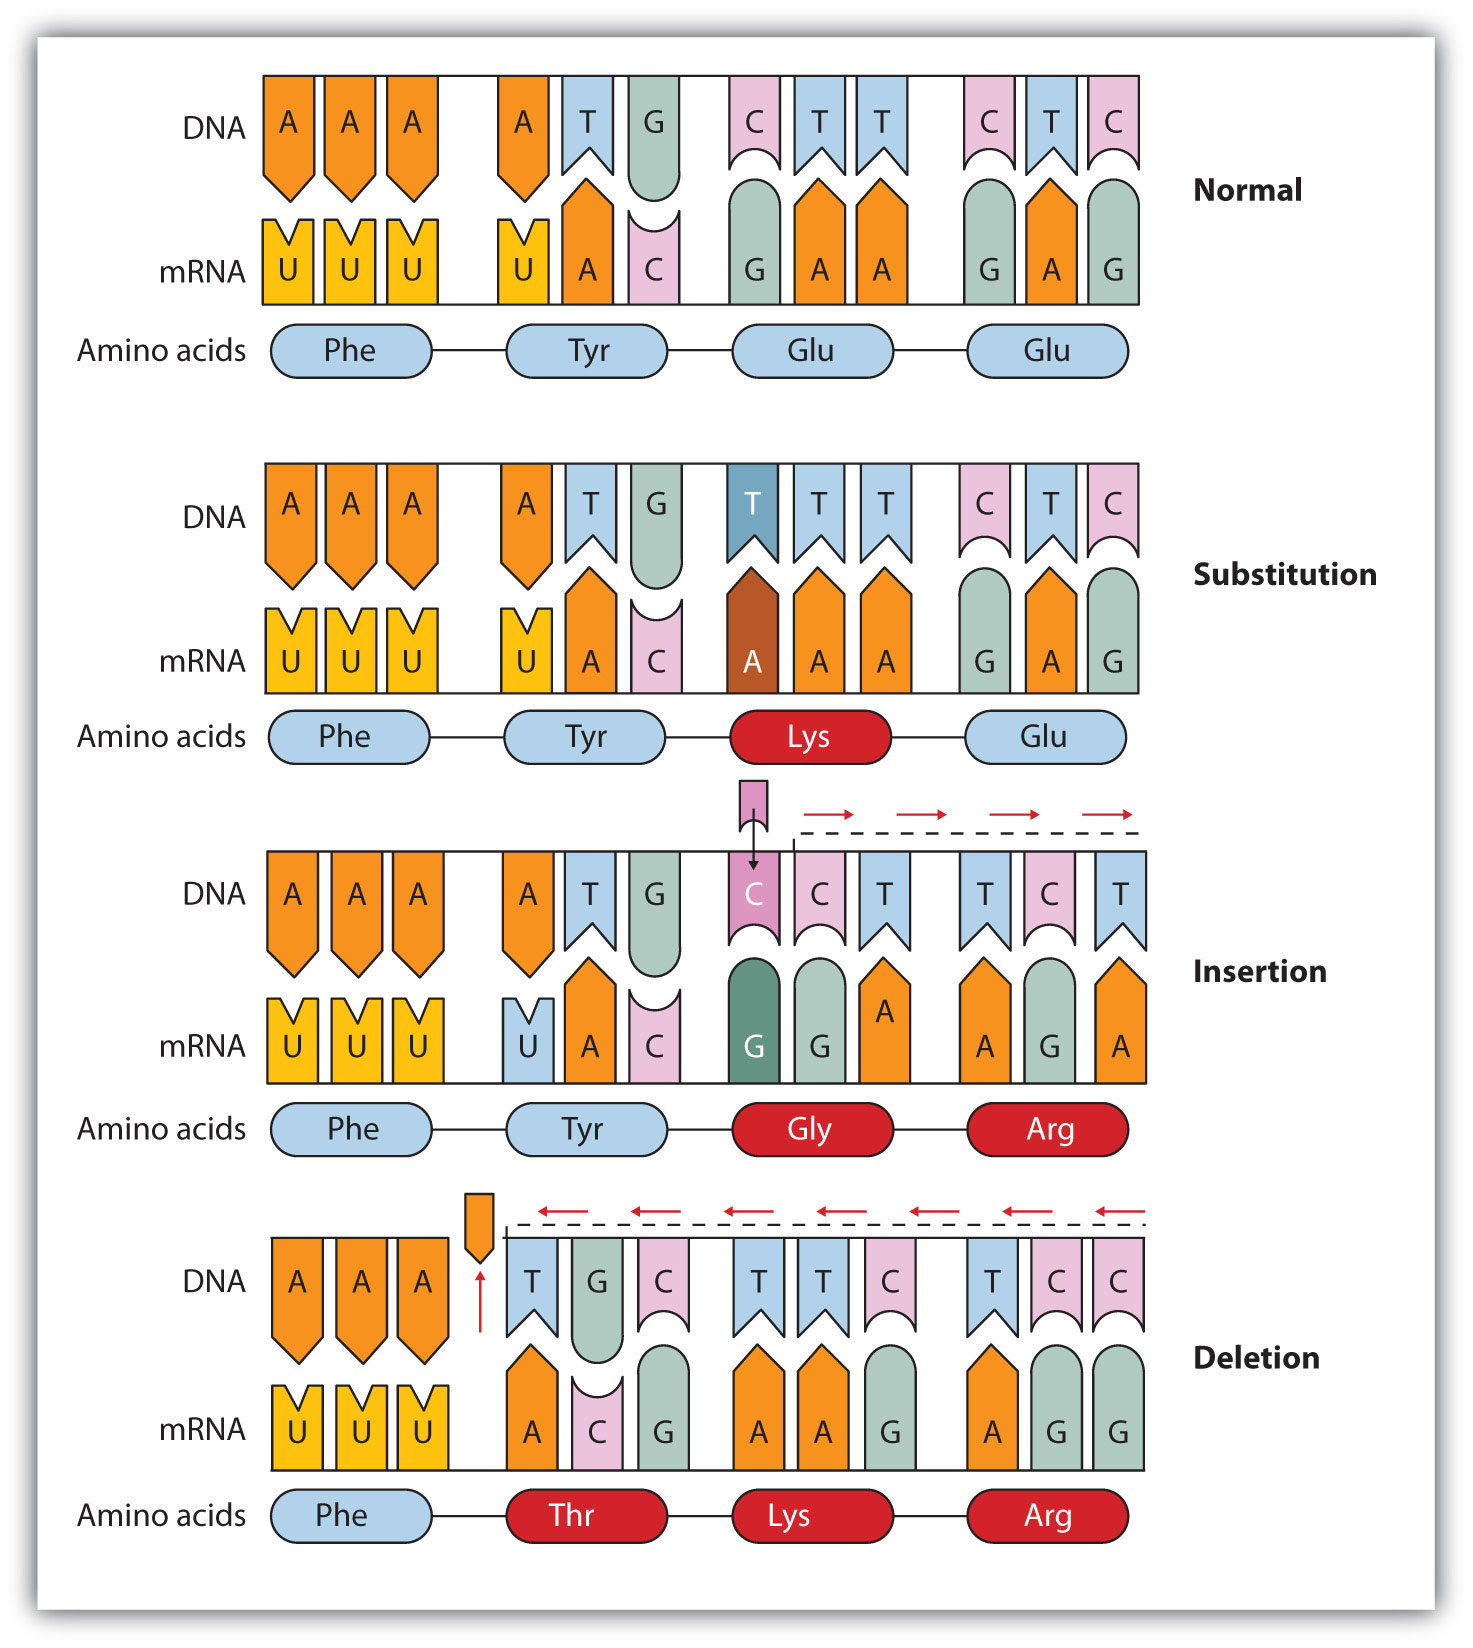
\includegraphics[width=0.7\textwidth]{../img/neoantigen/SNV}
	\caption{Ejemplos de SNV en el DNA. Fuente: \cite{socrates2022}}
	\label{fig:SNV}
\end{figure}

En la Figura \ref{fig:variants}, mostramos algunos tipos de SV. En este caso, también se pueden presentar INDELS, \textit{Tanden duplication}, inversiones, translocaciones y \textit{Copy Number Variants} (CNV). Los CNVs, representan fuertes candidatos para ser biomarcadores de varios tipos de Cáncer \citep{pan2019identification, lucito2007copy}. Otra mutación importante, es referente a la fusión de genes, en estos casos dos o más genes se fusionan y forman una proteína completamente diferente, este tipo de mutación también está fuertemente relacionado a varios tipos de Cáncer \citep{kerbs2022fusion, kim2019fusiongdb, heyer2020sequencing}.

\begin{figure}[h]
	\centering
	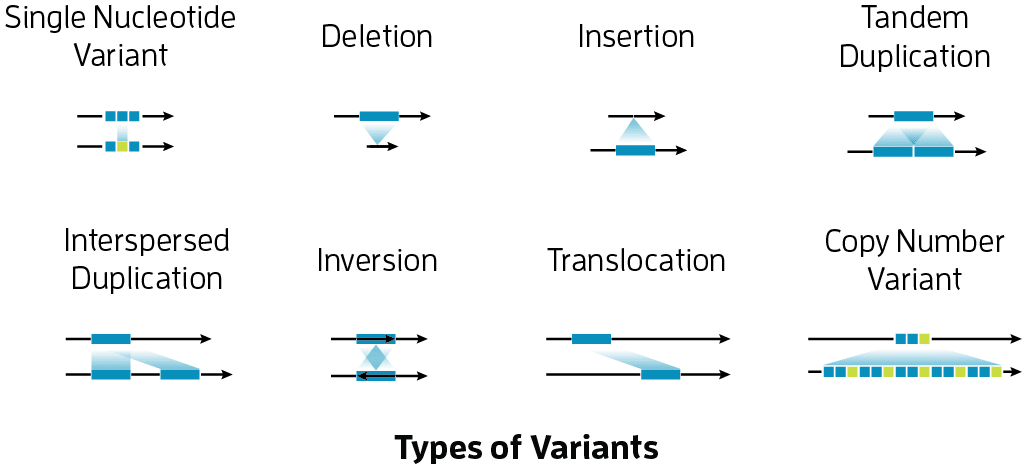
\includegraphics[width=0.7\textwidth]{../img/neoantigen/variants}
	\caption{Ejemplos de variaciones en el DNA. Fuente: \cite{sv_pacbio_2021}}
	\label{fig:variants}
\end{figure}


\subsection{Fusión de Genes}


Según \cite{williford2013gene}, la fusión de genes es un proceso mediante el cual las secuencias completas o parciales de dos o más genes distintos se fusionan en un solo gen, como resultado de reordenamientos derivados de ADN o ARN. Este fenómeno es ampliamente distribuido y se ha observado en todos los dominios de la vida. Además, la fusión de genes contribuyen de manera destacada al cambio evolutivo al proporcionar una fuente continua de nuevos genes. Las duplicaciones génicas a menudo preceden a las fusiones génicas, permitiendo la evolución de genes quiméricos, al mismo tiempo que preservan las funciones originales. A pesar de la reputación de las fusiones génicas como impulsores de la evolución adaptativa, pueden tener consecuencias devastadoras, a menudo dando lugar a trastornos genómicos o cáncer.

Las fusión de genes suelen ser causadas por alteraciones en la estructura genómica resultantes de daños en el ADN y por la posterior recombinación y replicación erróneas. Como se ve en la Figura \ref{fig:fusion}, las reorganizaciones genómicas pueden ocurrir entre uno o dos genes independientes a través de seis mecanismos conocidos: translocación, inserción, inversión, duplicación en tándem, eliminación y cromotripsis \citep{taniue2021fusion, dai2018fusion}.

Adicionalmente, la fusión de genes puede ser generada por eventos \textit{Trans-splicing} y \textit{Cis-splicing} (ver Figura \ref{fig:fusion2}). En \textit{Trans-splicing}, los exones de diferentes transcripciones de ARN se empalman y fusionan para producir un solo ARNm maduro. Otro mecanismo de empalmado es el \textit{Cis-splicing}, en el cual dos genes vecinos son transcritos en un solo ARN precursor mediante la lectura continua de la transcripción \citep{taniue2021fusion}.


\begin{figure}[h]
	\centering
	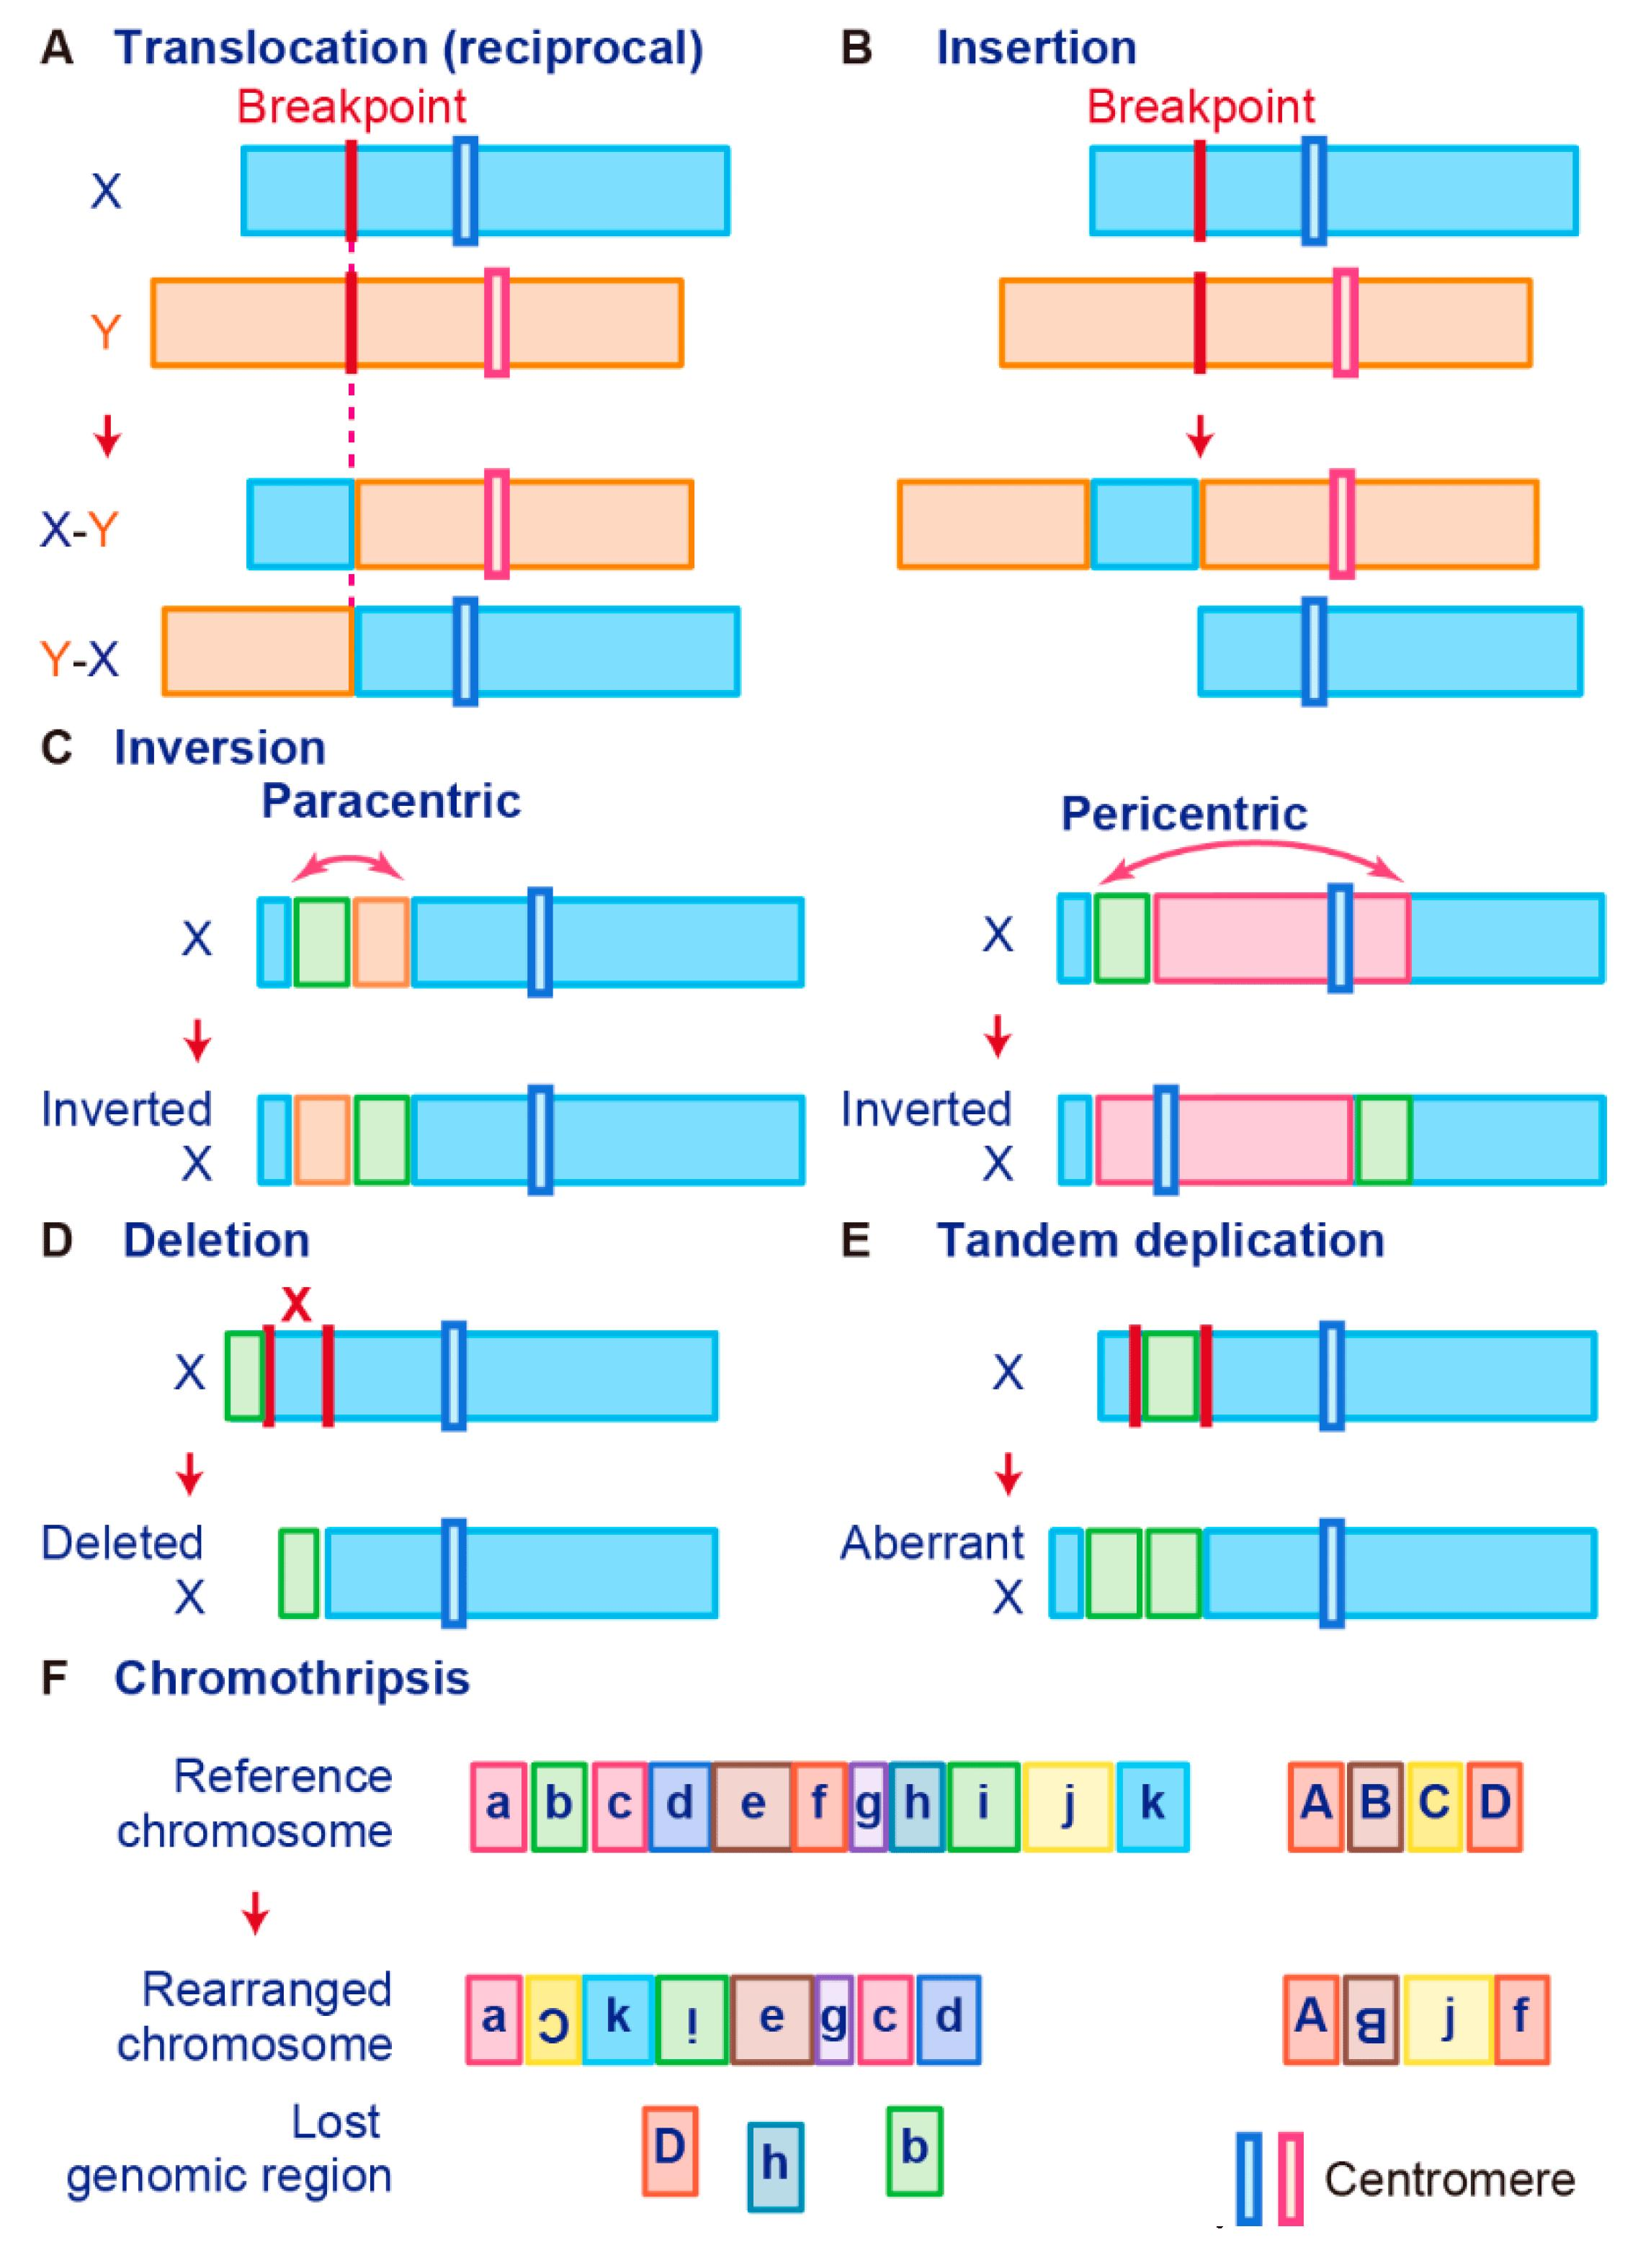
\includegraphics[width=0.7\textwidth]{../img/theory/fusion_gene}
	\caption[Representación de la fusión de genes.]{Representación esquemática de la formación de fusión de genes mediante reordenamientos cromosómicos estructurales. (A) Translocación. (B) Inserción. (C) Inversión. (D) Eliminación. (E) Duplicación en tándem. (F) Cromotripsis. Fuente: \cite{taniue2021fusion}}
	\label{fig:fusion}
\end{figure}


\begin{figure}[h]
	\centering
	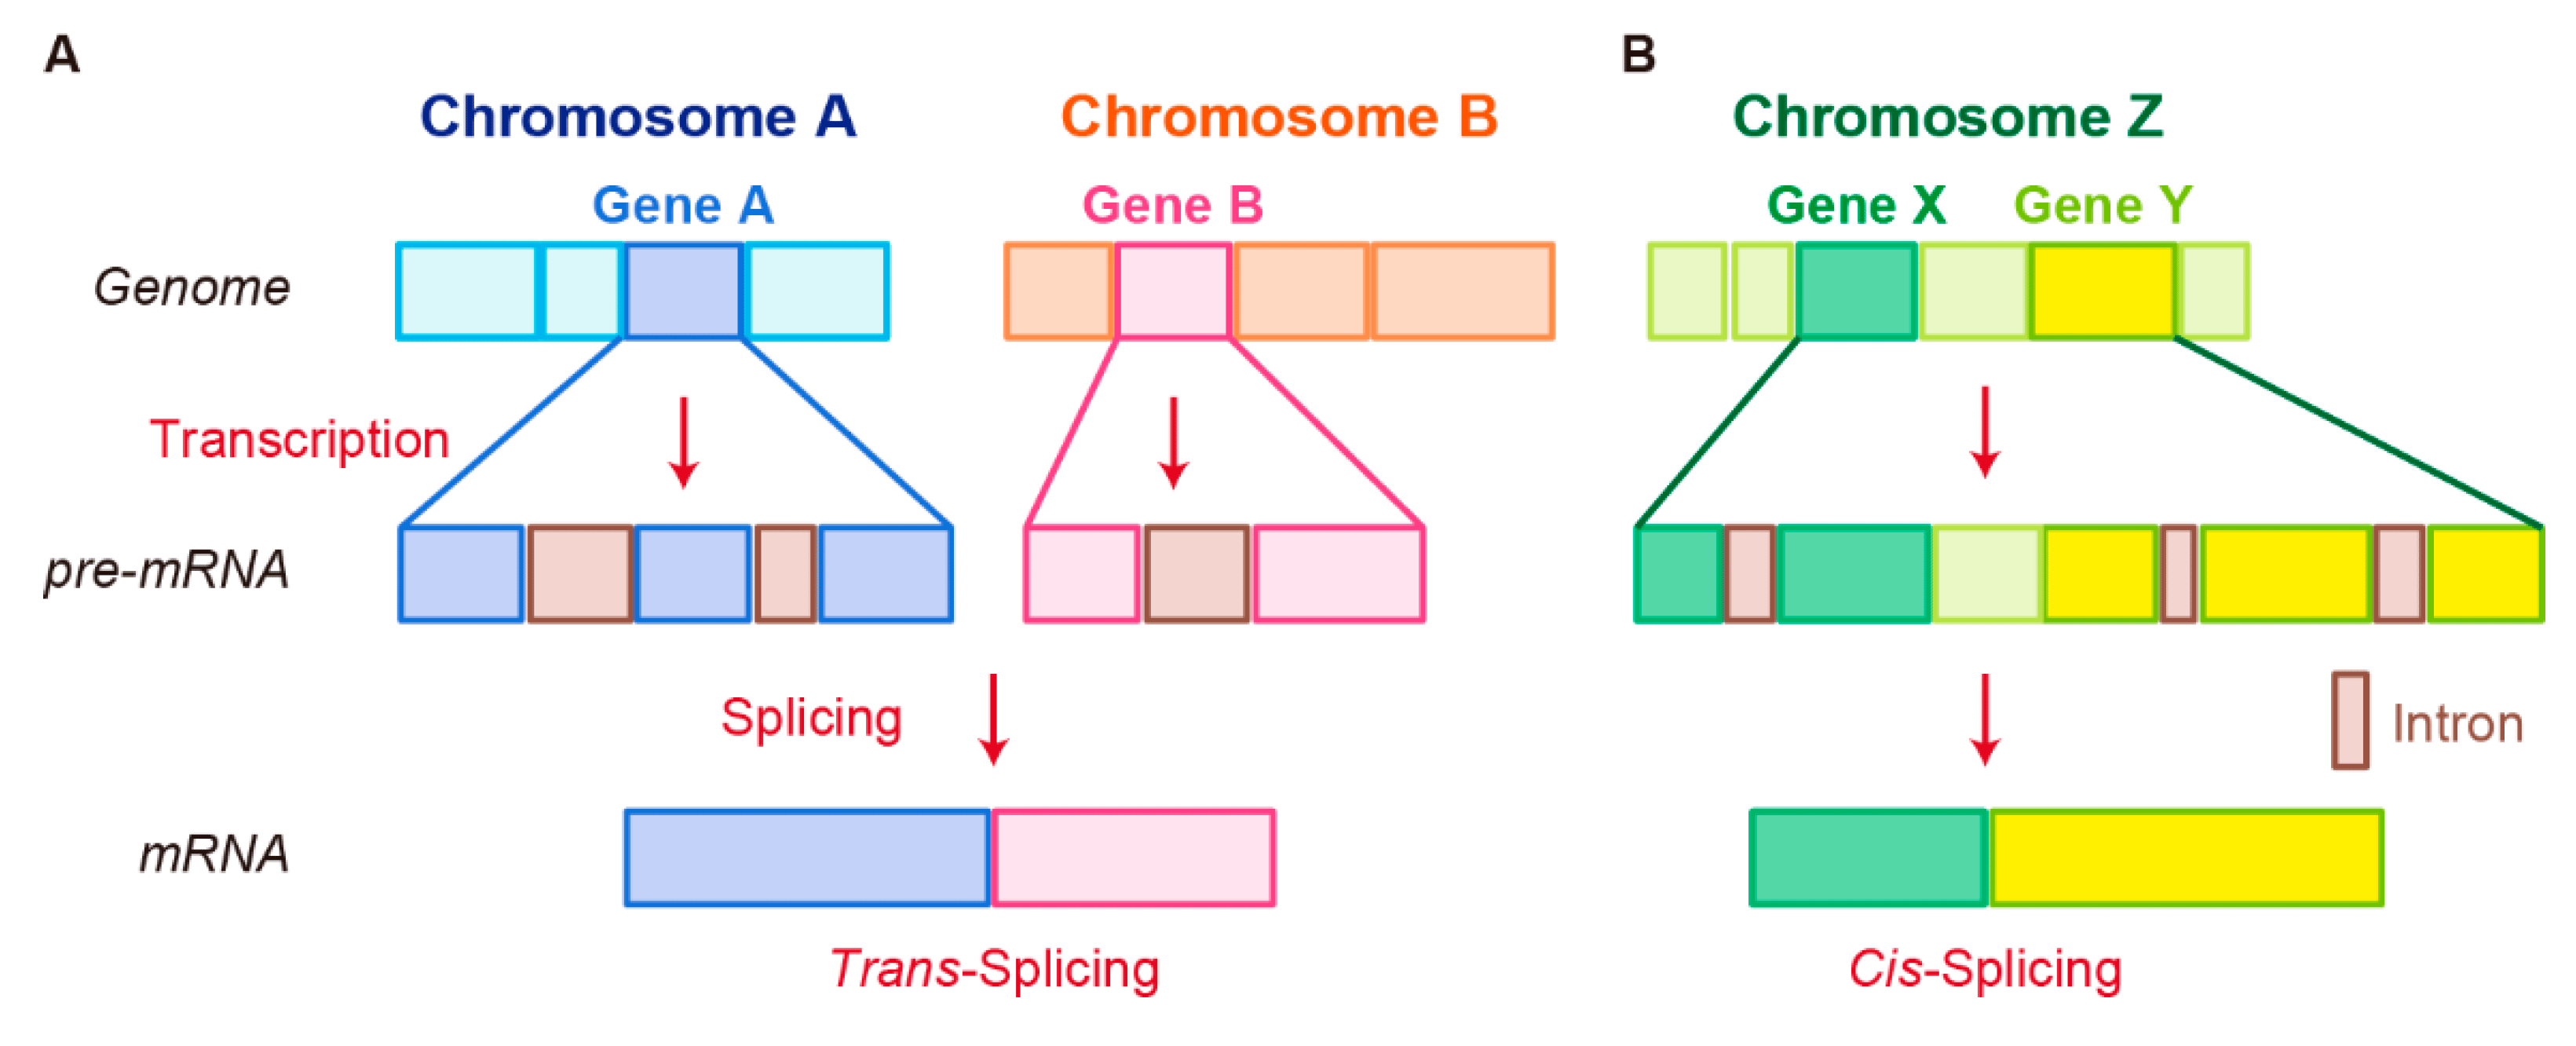
\includegraphics[width=0.85\textwidth]{../img/theory/fusion_gene2}
	\caption[Representación de \textit{Trans-splicing} y \textit{Cis-splicing}.]{Representación esquemática de la formación de ARN de fusión mediante reordenamientos cromosómicos no estructurales. (A) (A) \textit{Trans-splicing}. (B) \textit{Cis-splicing}. Fuente: \cite{taniue2021fusion}}
	\label{fig:fusion2}
\end{figure}


\section{Sistema Inmunitario}

El sistema inmunitario hace referencia al conjunto de células y procesos químicos que tiene como función protegernos de agentes extraños como: microbios, bacterias, células de Cáncer, toxinas, etc. \cite{marshall2018introduction}. En esta sección, se explicará de forma breve el comportamiento del sistema inmunitario frente cuando un agente extraño (antígeno) ingresa al cuerpo humano.

\subsection{Células T y APC}

Las células T también llamadas linfocitos T, se forman a partir de la médula ósea y son los encargados de eliminar agentes extraños (antígenos) \cite{NCIdictionary2022}. Estas células están compuestas por un \textit{T-cell Receptor} (TCR), que es el encargado de reconocer y enlazar a los antígenos. Luego, algunas células T, requieren de la acción de los \textit{Antigen Presenting Cells} (APC), estás células APC son: células dendríticas, macrófagos, células B, fibroblastos y células epiteliales. Normalmente, los APC devoran los antígenos y luego los presentan a las células T para su eliminación  \citep{marshall2018introduction}.


\subsection{MHC I y II}

Las proteínas \textit{Major Histocompatibility Complex} (MHC) I y II desempeñan un rol importante en el sistema inmunitario. Ambas proteínas tienen la función de presentar péptidos (antígenos) en la superficie de las células, para que sean reconocidas por la células T \citep{abualrous2021major}. MHC-I se encarga de la presentación de las células con núcleo, mientras que MHC-II, de las células APC. 

El proceso de presentación de los antígenos por MHC-I es el siguiente (Figura \ref{fig:mhc1}): la proteína foránea es degradado por el proteasoma y se producen péptidos (posibles antígenos), luego estos péptidos son transportados al \textit{Endoplasmic Reticulum} (ER) con la ayuda de \textit{Transporter associated Antigen Processing} (TAP), luego es migrado al aparato de Golgi para ser presentado en la superficie de la célula y es enlazado a la proteína MHC-I, una vez en la superficie, el antígeno puede ser reconocido por las células CD8+T \citep{zhang2019application}.




\begin{figure}[H]
	\centering
	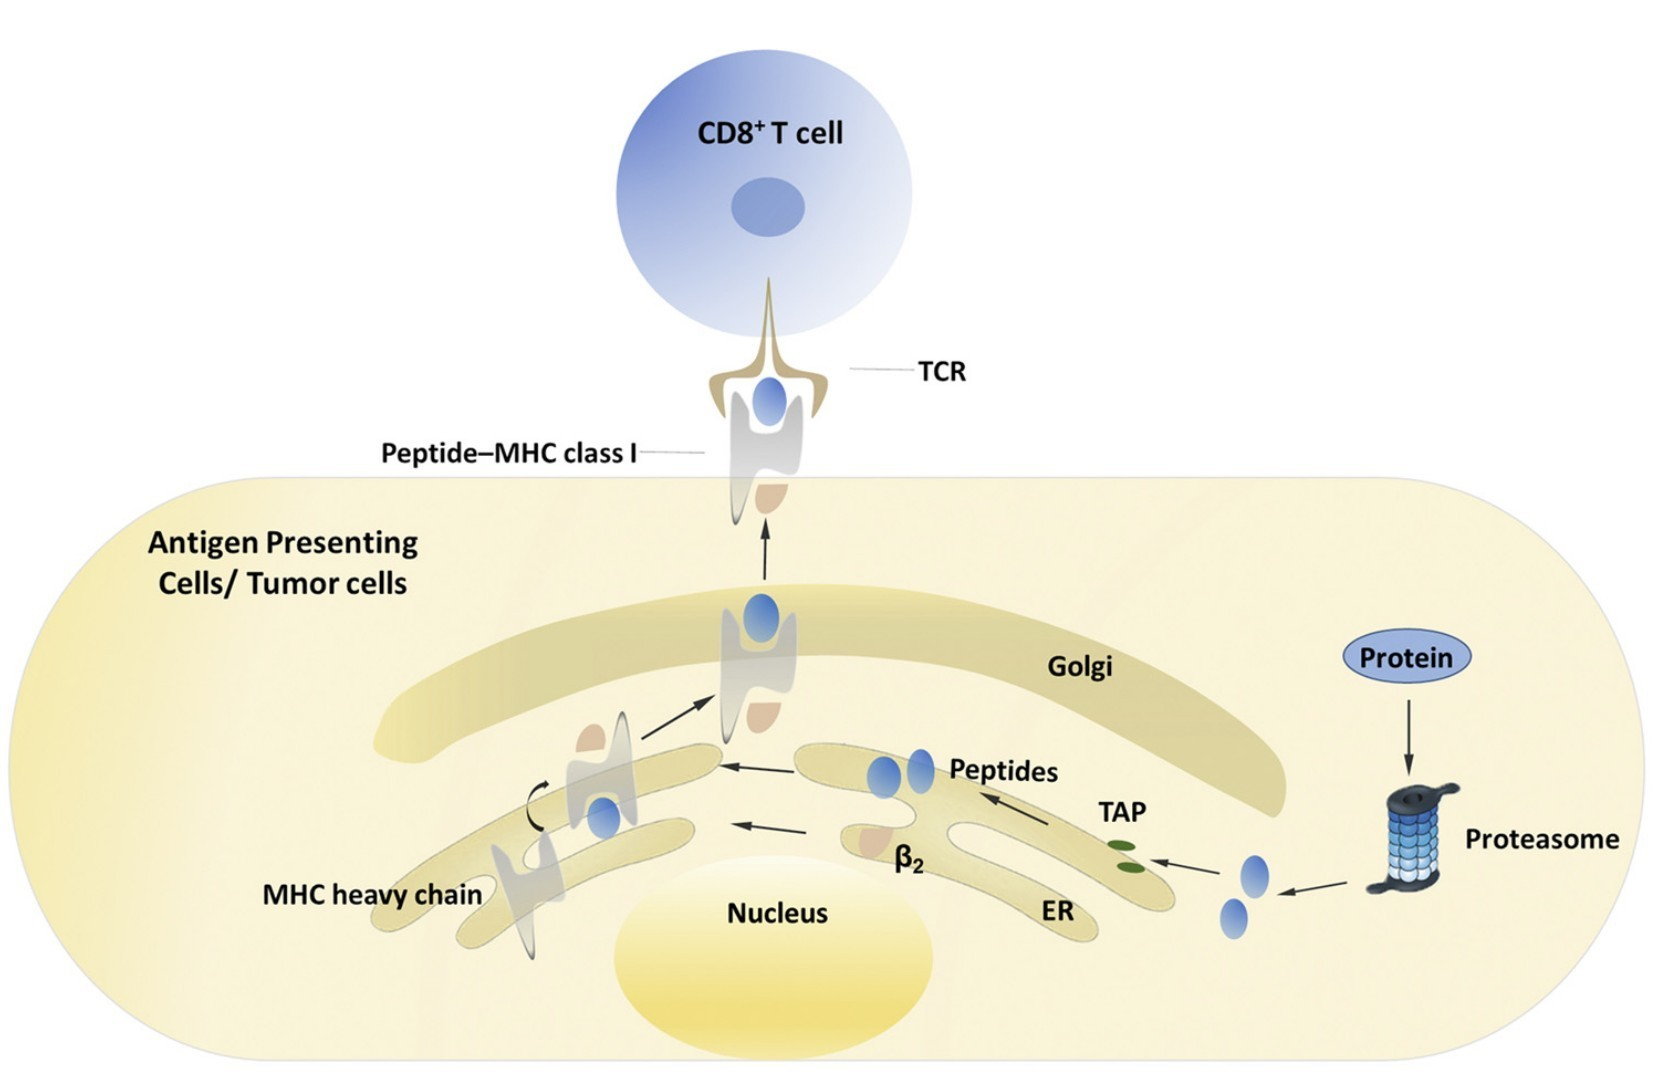
\includegraphics[width=0.8\textwidth]{../img/neoantigen/mhc1.jpg}
	\caption{Presentación de antígenos por MHC-I. Fuente: \cite{zhang2019application}}
	\label{fig:mhc1}
\end{figure}

Para el caso de MHC-II, es un proceso similar (Figura \ref{fig:mhc2}): primero, los patógenos son devorados por fagocitosis, los péptidos asociados a MHC-II son producidos en el \textit{Endoplasmic Reticulum} (ER), para luego ser trasladados al aparato de Golgi, y luego ser transportados a la superficie de las células una vez enlazadas con MHC-II, finalmente, son reconocidas por las células CD4+T \citep{zhang2019application}.



\begin{figure}[H]
	\centering
	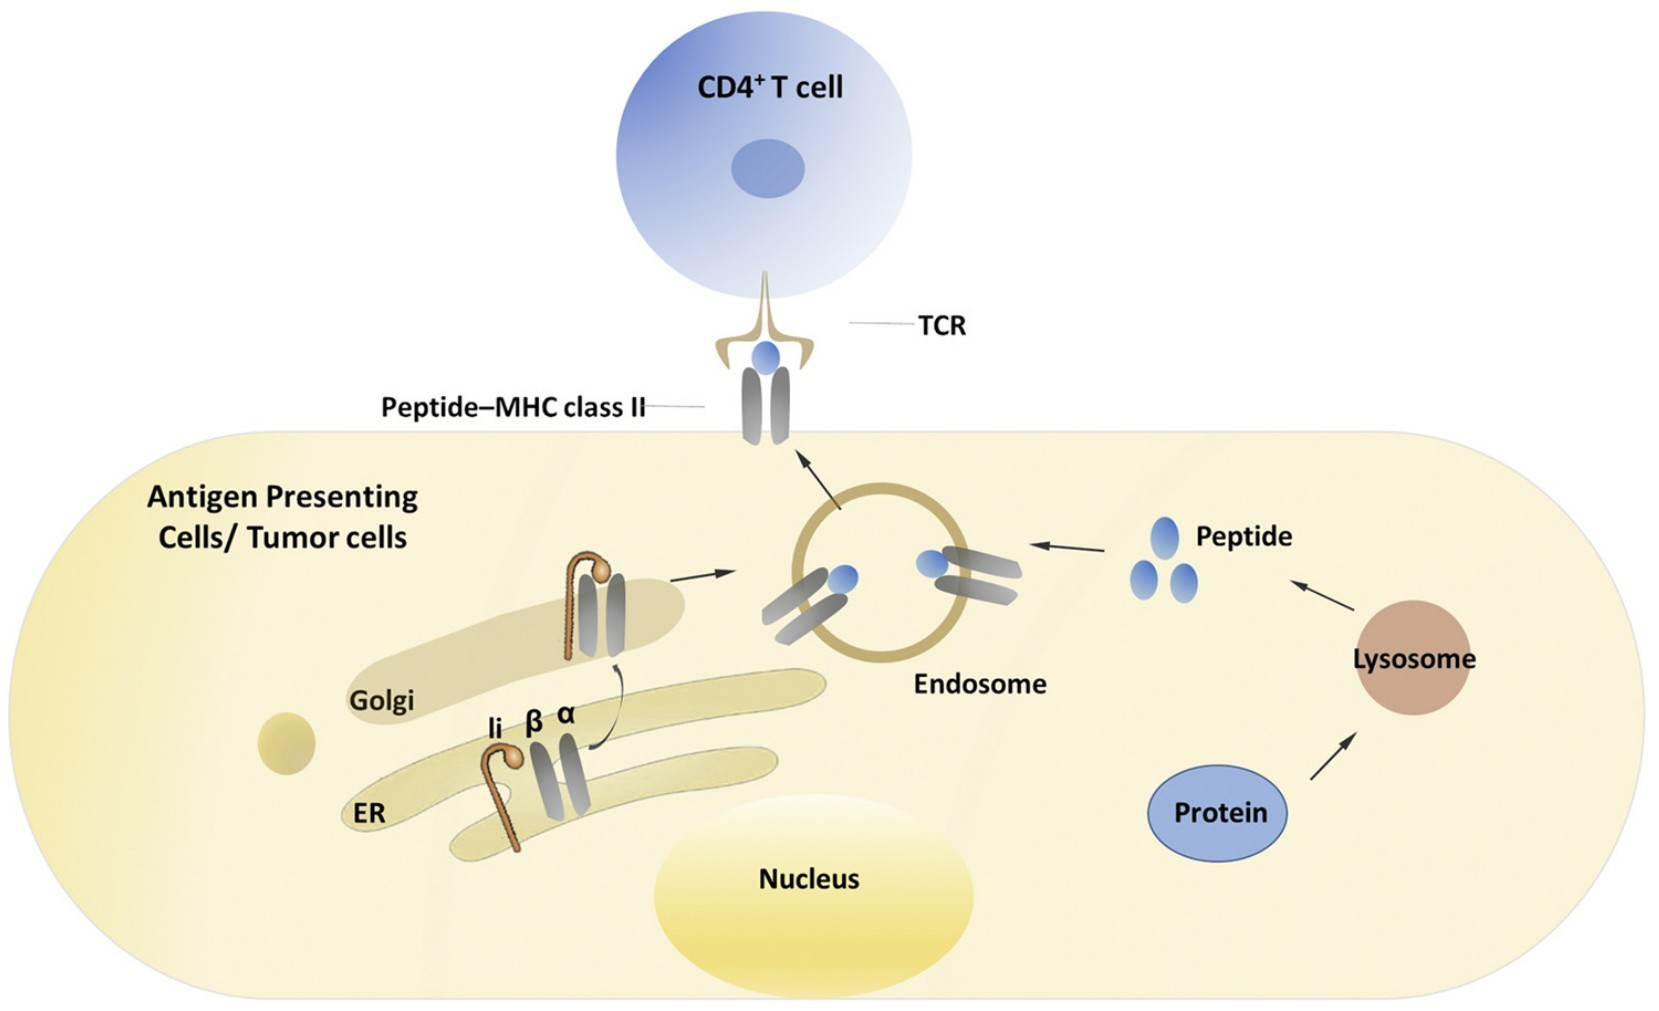
\includegraphics[width=0.8\textwidth]{../img/neoantigen/mhc2.jpg}
	\caption{Presentación de antígenos por MHC-II. Fuente: \cite{zhang2019application}}
	\label{fig:mhc2}
\end{figure}

\subsection{Neoantígenos}

Es una proteína que se forma en las células de Cáncer cuando ocurre mutaciones en el DNA. Los neo antígenos cumplen un rol importante al estimular una respuesta inmune en contra de células de Cáncer. En la actualidad, se estudia su uso en el desarrollo de vacunas contra el Cáncer \cite{NCIdictionary2022}. Una característica importante de los neo antígenos, es que solo están presentes en células tumorales y no en células sanas, debido a eso son considerados factores clave en la inmunoterapia del Cáncer \cite{borden2022cancer}. En la actualidad hay varios métodos para detectar a predecir neo antígenos, pero solo una pequeña porción de ellos logran estimular al sistema inmune \cite{chen2021challenges, hao2021improvement}.

 Este proceso para la detección de neo antígenos, generalmente consiste en: (1) extracción del tejido tumoral, (2) identificación de mutaciones, (3) detección de neo antígenos y predicción de inmunogenicidad, (4) desarrollo de experimentos \textit{in vitro} y (5) desarrollo de la vacuna \citep{de2020neoantigen, peng2019neoantigen} (ver Figura \ref{fig:process}). 

\begin{figure}[H]
	\centering
	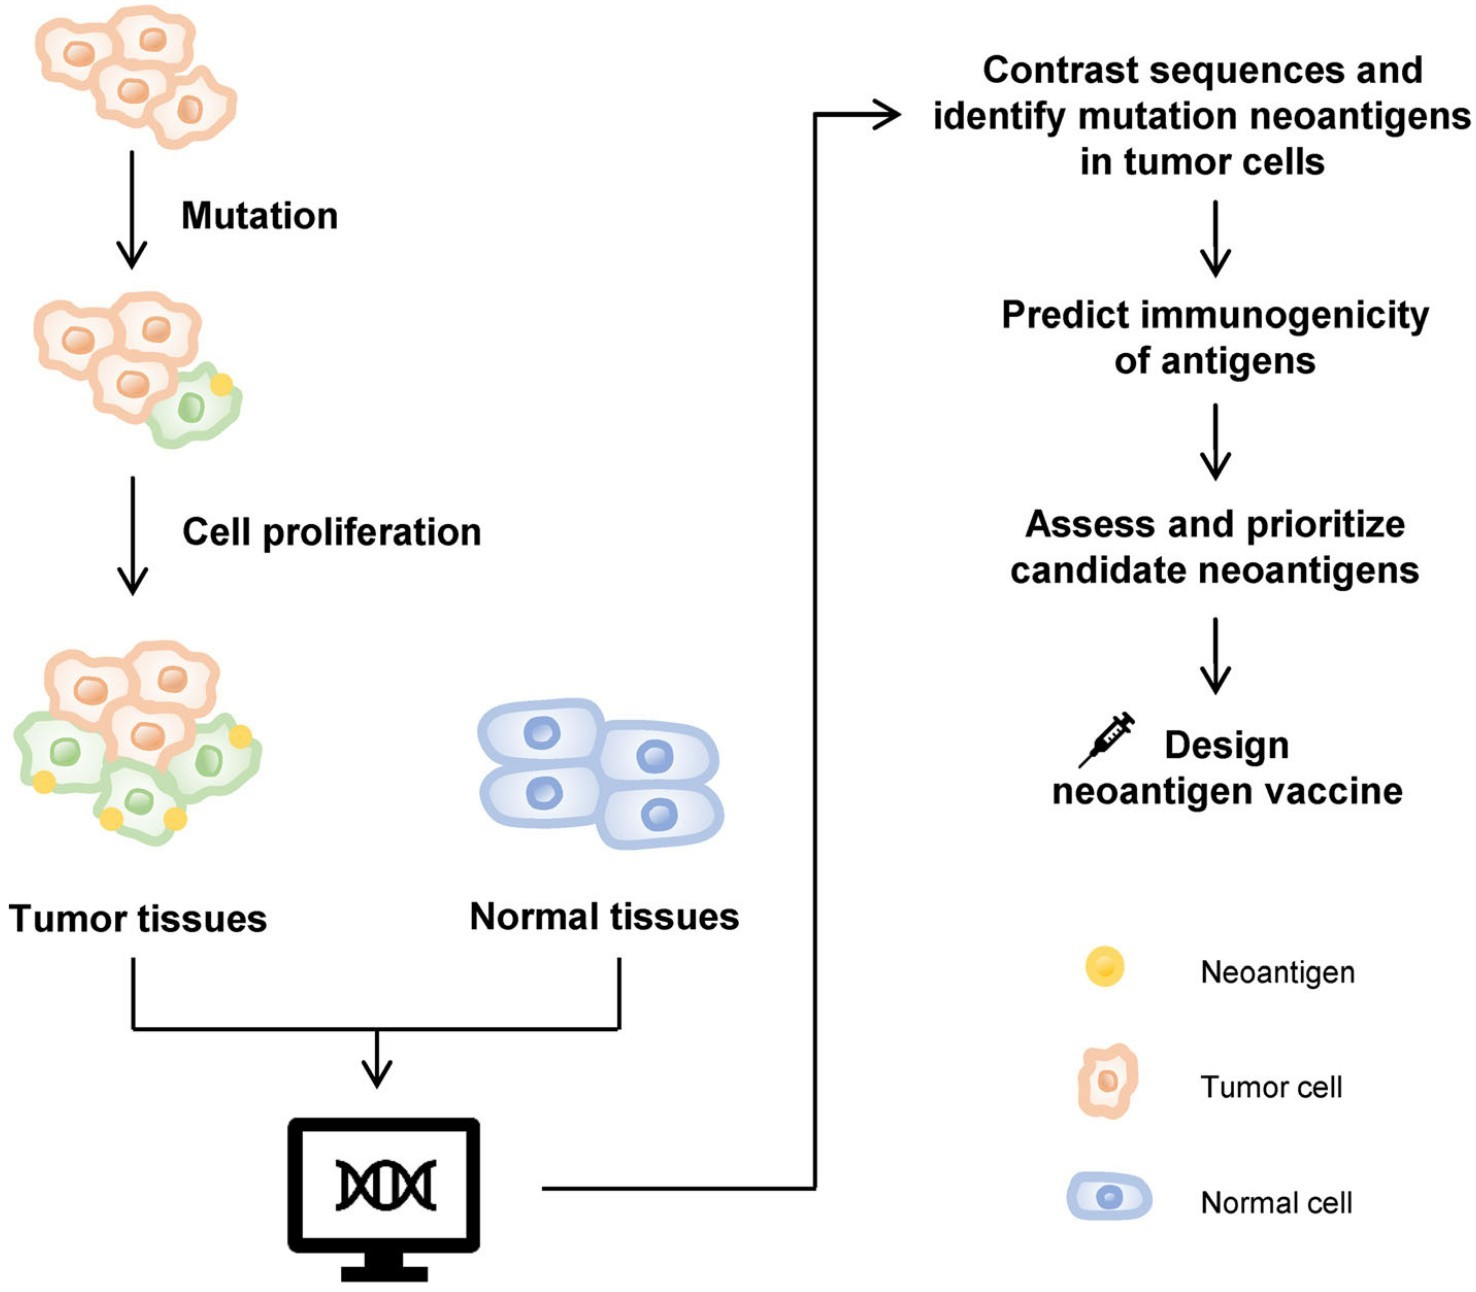
\includegraphics[width=0.7\textwidth]{../img/neoantigen/process}	
	\caption{Proceso para la detección de neo antígenos y generación de vacunas personalizadas. Fuente: \citep{de2020neoantigen} }
	\label{fig:process}
\end{figure}


\subsection{Inmunoinformática}

Según \cite{tong2009immunoinformatics}, la Inmunoinformática,  combina la inmunología tradicional con ciencias de la computación, matemáticas, química, bioquímica, genómica y proteómica para el análisis a gran escala de la función del sistema inmunológico, ofrece nuevas oportunidades para la investigación futura, desde el laboratorio hasta el paciente. Gracias a las nuevas tecnologías y algoritmos en las Ciencias de la Computación, este campo ha generado bastante investigación y promete ser una área de riguroso estudio en el futuro. Además, esta tesis se sitúa en este campo de estudio, al aplicar metodologías de Inteligencia Artificial a la Inmunología.

\section{\textit{Machine Learning}}

\textit{Machine Learning} (ML) es una categoría de algoritmos computacionales capaces de emular algunas acciones inteligentes. Es el resultado de varias disciplinas como: inteligencia artificial, probabilidad, estadística, ciencia de la computación, teoría de la computación, psicología y filosofía \citep{el2022machine}. \textit{Machine Learning}  tiene varias definiciones, pero una de las mas acertadas, según \cite{samuel1967some}: ``Campo de estudio que brinda a las computadoras la habilidad de aprender sin haber sido explícitamente programado''. \\





\subsection{Algoritmos de Aprendizaje}

Un algoritmo de aprendizaje o \textit{machine learning algorithm}, es aquel algoritmo que no debe ser programado explícitamente, este aprende de la experiencia, a partir de datos \citep{Goodfellow2016}.  Según \cite{mitchell1997machine}: \textit{``A computer program is said to learn from experience \textit{E} with respect to some class of tasks \textit{T} and performance measure \textit{P}, if its performance at tasks in \textit{T}, as measured by \textit{P}, improves with experience \textit{E}''}. La traducción a español indicaría: ``Un programa de computadora puede aprender de una experiencia \textit{E}, para una tarea \textit{T} y con una métrica de desempeño \textit{P}, si el desempeño de la tarea \textit{T}, medido con \textit{P}, mejorar con la experiencia \textit{E}''. Esto, nos da a entender que un programa de computadora puede aprender si mejora su desempeño según aumente su experiencia o datos.



\subsubsection{La Tarea, \textit{T}}

La tarea \textit{T} de ML, puede ser descrito como de la forma en que el sistema de ML procesa una muestra o ejemplo. Según \cite{Goodfellow2016} las tareas más comunes de ML son:

\begin{itemize}
	\item \textbf{Clasificación}. En este caso, el algoritmo de ML debe predecir la clase a la que pertenece la muestra como una función: $f: \mathbb{R}^n \rightarrow \{ 1, ..., k \}$. También puede escribirse como: $y = f(x)$, aquí $x$ representa la entrada y la función $f$ determinará la clase a la que pertenece.
	
	\item \textbf{Regresión}.  El algoritmo debe producir una función: $f: \mathbb{R}^n \rightarrow \mathbb{R}$. Es decir, dada como entrada un vector $x$ de números reales, el algoritmo de ML debe predecir un valor en los números reales.
	
	\item \textbf{Transcripción}. En este caso, dada como entrada datos no estructurados, el algoritmo de ML debe generar información de forma textual. Por ejemplo: dada una imagen como entrada, la salida sería el texto encontrado en la imagen.
	
	\item \textbf{Maquinas de traducción}. Como el nombre indica, la entrada es un texto en un lenguaje y la salida es un texto en otro lenguaje.
	
	\item \textbf{Salida estructurada}. En este caso la salida es un vector o alguna estructura de datos de varios valores. El procesamiento natural de lenguaje es un buen ejemplo, la entrada es un texto y la salida es un árbol que denota la estructura gramatical y semántica de la entrada.
	
	\item \textbf{Detección de anomalías}. En este tipo de problemas el algoritmo de ML, busca detectar eventos anómalos, es decir muestras que no corresponden a la distribución normal de los datos. Un ejemplo, es la detección de transacciones fraudulentas.
	
	\item \textbf{Síntesis y muestreo}. En este caso, el algoritmo de ML debe generar nuevas muestras a partir de un conjunto de entrenamiento. Esto se aplica en los videojuegos, para la generación automática de texturas para objetos de gran tamaño.
	
	
	

\end{itemize}

\subsubsection{El Desempeño, \textit{P}}


Es muy importante medir el desempeño de un algoritmo de ML, usualmente la métrica utilizada puede variar según la tarea \textit{T}. Para tareas de clasificación, usualmente se suele aplicar \textit{Precision} y \textit{Recall}, estos están detallados en las Ecuaciones \ref{eq:presicion} y \ref{eq:recall} respectivamente \citep{dalianis2018evaluation}.


\begin{equation} \label{eq:presicion}
	\mbox{\textit{Precision: }} P = \frac{tp}{tp + fp}
\end{equation}

\begin{equation} \label{eq:recall}
	\mbox{\textit{Recall: }} R = \frac{tp}{tp + fn}
\end{equation}

donde \textit{tp}, hace referencia a la cantidad de muestras que eran verdaderas y han sido reconocidas como verdaderas; \textit{fp}, son las muestras que eran falsas, pero fueron reconocidas como verdaderas; \textit{fn}, son las muestras que eran negativas y fueron reconocidas como negativas. Otra métrica importante es el \textit{F-score}, este puede ser definido como el peso promedio de \textit{Precision} y \textit{Recall}  \citep{dalianis2018evaluation}. En la Ecuación \ref{eq:fbeta}, presentamos la definición.


 
\begin{equation} \label{eq:fbeta}
	\mbox{\textit{F-score: }} F_\beta = (1 + \beta^2) * \frac{P*R}{\beta^2*P + R}
\end{equation}

Cuando $\beta = 1$:
 
\begin{equation} \label{eq:f1}
	\mbox{\textit{F-score: }} F_1 = 2 * \frac{P*R}{P + R}
\end{equation}

Finalmente otra métrica, aunque no muy recomendada para datos no balanceados es el \textit{accuracy}. Este representa el porcentaje de muestras reconocidas correctamente.

\begin{equation} \label{eq:f1}
	\mbox{\textit{Accuracy: }} acc = \frac{tp + tn}{ tp +tn +fp +fn}
\end{equation}


Para otro tipo de problemas, como regresión se puede aplicar el \textit{error rate}, esta es una medida en los números reales y nos indica que tan diferente es la predicción realizada por un algoritmo de ML \citep{Goodfellow2016}.


\subsubsection{La Experiencia, \textit{E}}

Según el tipo de experiencia que realizan los algoritmos de ML, se pueden clasificar en: Aprendizaje supervisado y Aprendizaje no supervisado \cite{Goodfellow2016}.

\begin{itemize}
	\item \textbf{Aprendizaje supervisado}. En este caso, cada muestra par el entrenamiento tiene los datos de entrada $x$ y una etiqueta $l$. La idea es que el algoritmo de ML, pueda aprender de estos datos y luego realizar predicción de la etiqueta $j$ tomando como entrada sólo los datos $x$. Según, \cite{prince2023understanding} los modelos de aprendizaje supervisado definen una relación entre los datos de entrada y una predicción de salida. Generalmente, podemos en esta área tenemos tratamos problemas de regresión y clasificación. El primero predice un número real mientras que el otro clasifica a un tipo de clase.
	
	\item \textbf{Aprendizaje no supervisado}. En este caso, solo se cuenta con muestras no etiquetadas. Entonces el algoritmo   de ML, debe agrupar los datos en \textit{clusters}. Un ejemplo de estos problemas es la segmentación de clientes, segmentación de noticias, etc. Adicionalmente, tenemos los modelos generativos, que aprenden a sintetizar nuevos ejemplos de datos que son estadísticamente indistinguibles de los datos de entrenamiento. Algunos modelos generativos describen explícitamente la distribución de probabilidad sobre los datos de entrada, y nuevos ejemplos se generan muestreando de esta distribución. Otros simplemente aprenden un mecanismo para generar nuevos ejemplos sin describir explícitamente su distribución \citep{prince2023understanding}.
	
	\item \textbf{Aprendizaje por refuerzo}. La última área de aprendizaje automático es el aprendizaje por refuerzo. Este paradigma introduce la idea de un agente que vive en un mundo y puede realizar ciertas acciones en cada paso de tiempo. Las acciones cambian el estado del sistema, pero no necesariamente de manera determinista. Tomar una acción también puede producir recompensas, y el objetivo del aprendizaje por refuerzo es que el agente aprenda a elegir acciones que conduzcan a altas recompensas en promedio \citep{prince2023understanding}.
	
\end{itemize}


En la Figura \ref{fig:ml} disponemos de los tipos de aprendizaje en ML. Pueden dividirse de manera general en aprendizaje supervisado, aprendizaje no supervisado y aprendizaje por refuerzo. Las redes neuronales profundas contribuyen a cada una de estas áreas \cite{prince2023understanding}.

\begin{figure}[H]
	\centering
	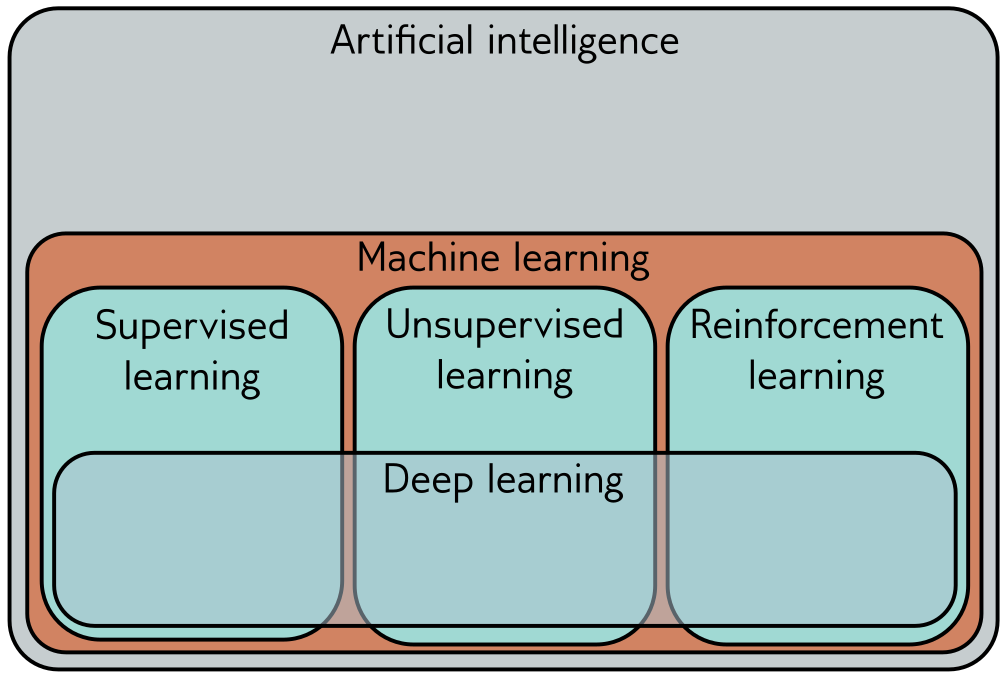
\includegraphics[width=0.6\textwidth]{../img/theory/ml}	
	\caption{Tipos de aprendizaje en \textit{Machine Learning}. Fuente: \citep{prince2023understanding} }
	\label{fig:ml}
\end{figure}



% queda pendiente hablar sobre regresión lineal, logistica y redes neuronales


\subsection{Redes Neuronales}

Uno  de los modelos mas representativos de ML son la redes neuronales. Estas se basan en unidades llamadas neuronas (perceptrón). En la Figura \ref{fig:neuron}, se muestra esta representación, donde $x_i$, representa un atributo, $w_i$ es el peso que se asigna al atributo $x_i$, de esta forma la neurona representa el resultado de multiplicar un peso a un atributo: $\sum_{i=1}^{d} x_i \cdot w_i$, una representación vectorial sería: $\textbf{x}^T\textbf{w}$ \citep{nielsen2015neural}. Luego, a dicho resultado se aplica una función de activación, la función mas utilizada es la función sigmoidea (Ecuación \ref{eq:sigmoidea} y \ref{eq:sigmoidea2}).  

\begin{equation}\label{eq:sigmoidea}
	\sigma (z) = \frac{1}{1 + e^{-z}}
\end{equation}

donde $z = \sum_{i}^{} w_i \cdot x_i - b$.

\begin{equation}\label{eq:sigmoidea2}
	\frac{1}{1 + e^{-\sum_{i}^{} w_i \cdot x_i - b}}
\end{equation}

%Pero, existen otras funciones de activación que se pueden aplicar según el problema: Softmax: $\phi(x) = \frac{e^{x_i}}{\sum_{j=0...k^{e^{x_j}}} }; i = 0, 1, 2, ..., k$, función tangente hiperbolica: $\phi(x) = \frac{e^x - e^{-x}}{e^x + e^{-x}}$ y RELU: $\phi(x) = max(0, x)$.

\begin{figure}[H]
	\centering
	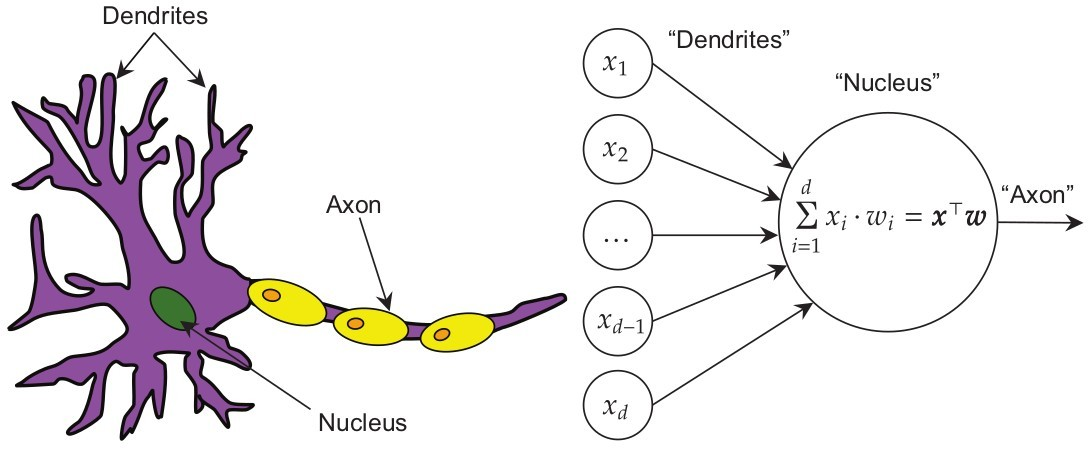
\includegraphics[width=0.8\textwidth]{../img/neoantigen/neuron}
	\caption{Representación de una neurona. Fuente: \cite{insideDL2022}.}
	\label{fig:neuron}
\end{figure}

El perceptrón, es capaz de solucionar varios problemas, pero para casos complejos puede formar una red, como se presenta en la Figura \ref{fig:nn}.

\begin{figure}[H]
	\centering
	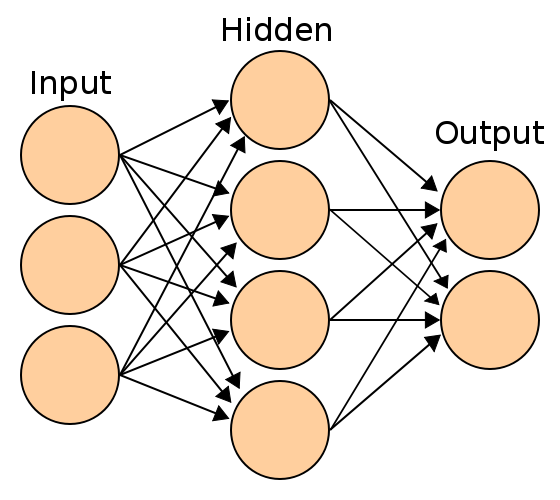
\includegraphics[width=0.35\textwidth]{../img/neoantigen/nn2}
	\caption{Representación de una red neuronal. }
	\label{fig:nn}
\end{figure}

En resumen, para la red neuronal de la Figura \ref{fig:shallow}, una red neuronal con una entrada escalar $x$, cuatro unidades ocultas $h_1, h_2, h_3, h_4$, y una salida 2D $y = [y_1, y_2]^T$, se define con las Ecuaciones \ref{equa:ml_1} y \ref{equa:ml_2}. Además, $a[\bullet]$ es la función de activación, generalmente para las capas ocultas es representada por la función ReLU.

\begin{equation}\label{equa:ml_1}
	\begin{split}
	h_1 = a [ \theta_{10} + \theta_{11}x  ]	 \\	
	h_2 = a [ \theta_{20} + \theta_{21}x  ]	 \\
	h_3 = a [ \theta_{30} + \theta_{31}x  ]	 \\
	h_4 = a [ \theta_{40} + \theta_{41}x  ]	 
	\end{split}
\end{equation}	

\begin{equation}\label{equa:ml_2}	
	\begin{split}
		y_1 = \phi_{10} + \phi_{11}h_1  + \phi_{12}h_2 + \phi_{13}h_3 + \phi_{14}h_4 \\
		y_2 = \phi_{20} + \phi_{21}h_1  + \phi_{22}h_2 + \phi_{23}h_3 + \phi_{24}h_4
	\end{split}
\end{equation}	

\begin{figure}[H]
	\centering
	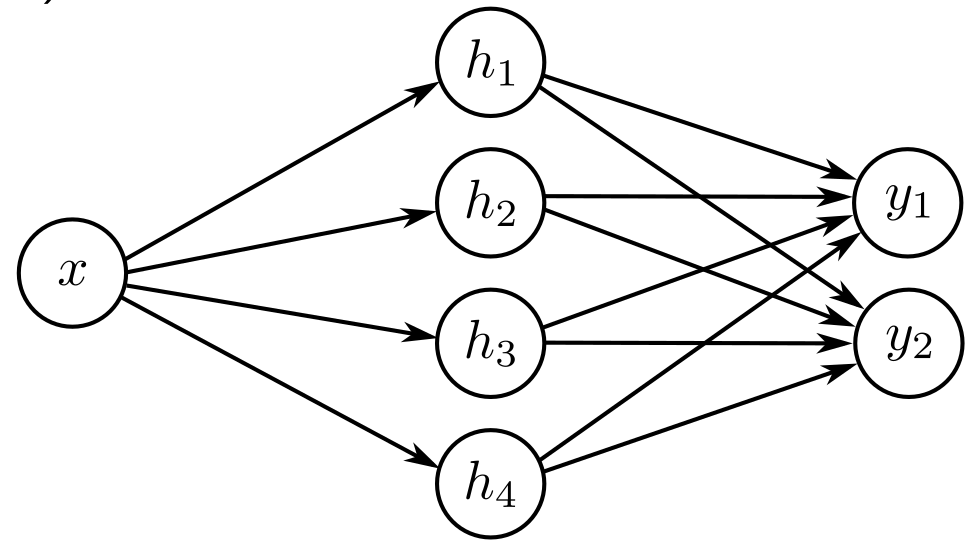
\includegraphics[width=0.5\textwidth]{../img/theory/shallow}
	\caption{Red neuronal con una entrada, cuatro unidades ocultas y dos salidas. Fuente: \cite{prince2023understanding} }
	\label{fig:shallow}
\end{figure}

\section{\textit{Deep Learning}}

\textit{Deep learning} (DL) es una subcategoría de \textit{Machine Learning}, a diferencia de los algoritmos tradicionales de ML, usualmente DL trata con señales sin pre-procesamiento, los modelos (basados en redes neuronales) son mucho mas complejos tanto en dimensión como en el método de aprendizaje \citep{el2022machine}. Por ejemplo, en la Figura \ref{fig:dl}, presentamos la relación entre Inteligencia Artificial (IA), ML y DL, de ahí podemos concluir que ML es parte de la IA y DL es parte de ML \citep{el2022machine}.

\begin{figure}[H]
	\centering
	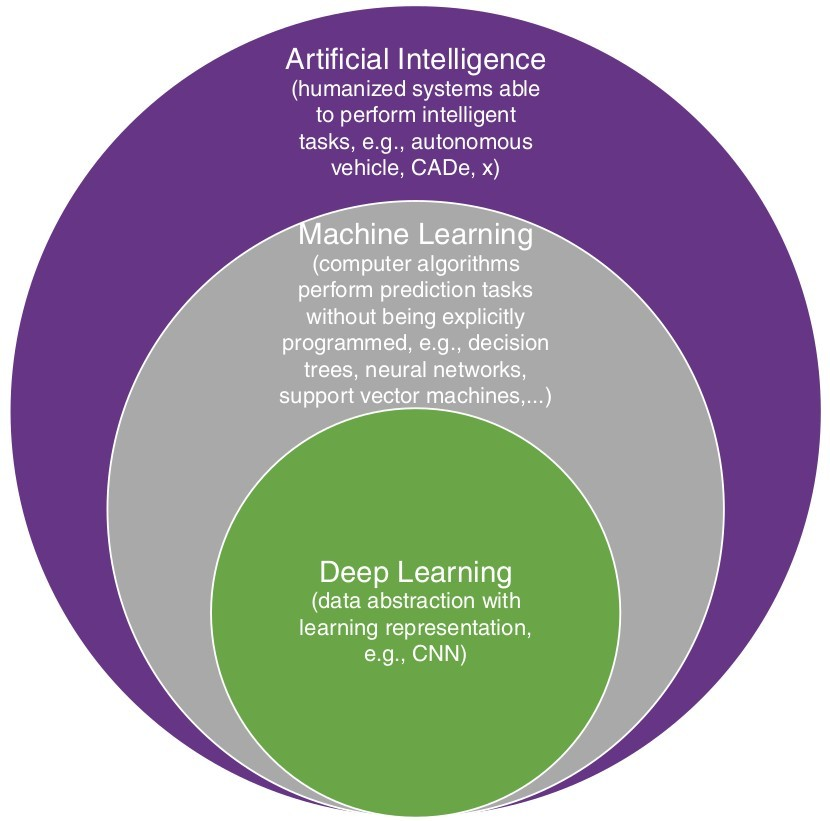
\includegraphics[width=0.5\textwidth]{../img/neoantigen/dl}
	\caption{Relación entre Inteligencia Artificial, \textit{Machine Learning} y \textit{Deep Learning}. Fuente: \cite{el2022machine}.}
	\label{fig:dl}
\end{figure}

Además, a medida que aumenta el número de unidades ocultas, las redes neuronales  mejoran su capacidad descriptiva. De hecho, con suficientes unidades ocultas, las redes  pueden describir funciones arbitrariamente complejas. Sin embargo, resulta que para algunas funciones, el número necesario de unidades ocultas es prácticamente grande \cite{prince2023understanding}. 




\subsection{Redes Neuronales Profundas}

\textit{Deep Neural Networks} o Redes Neuronales Profundas,  son perceptrones multicapa o \textit{multilayer perceptrons}(MLP). Su objetivo es aproximar una función $f^*$, para el caso de clasificación, podría modelarse como $ y=f^*(x)$. Luego, un \textit{feedforward network}, define un mapeo $y = f(x;\theta)$ y aprende los valores de los parámetros $\theta$ \cite{Goodfellow2016}. Entonces una red neuronal profunda, es una red neuronal tradicional pero con un número grande de neuronas y capas (Figura \ref{fig:dnn}). 

\begin{figure}[]
	\centering
	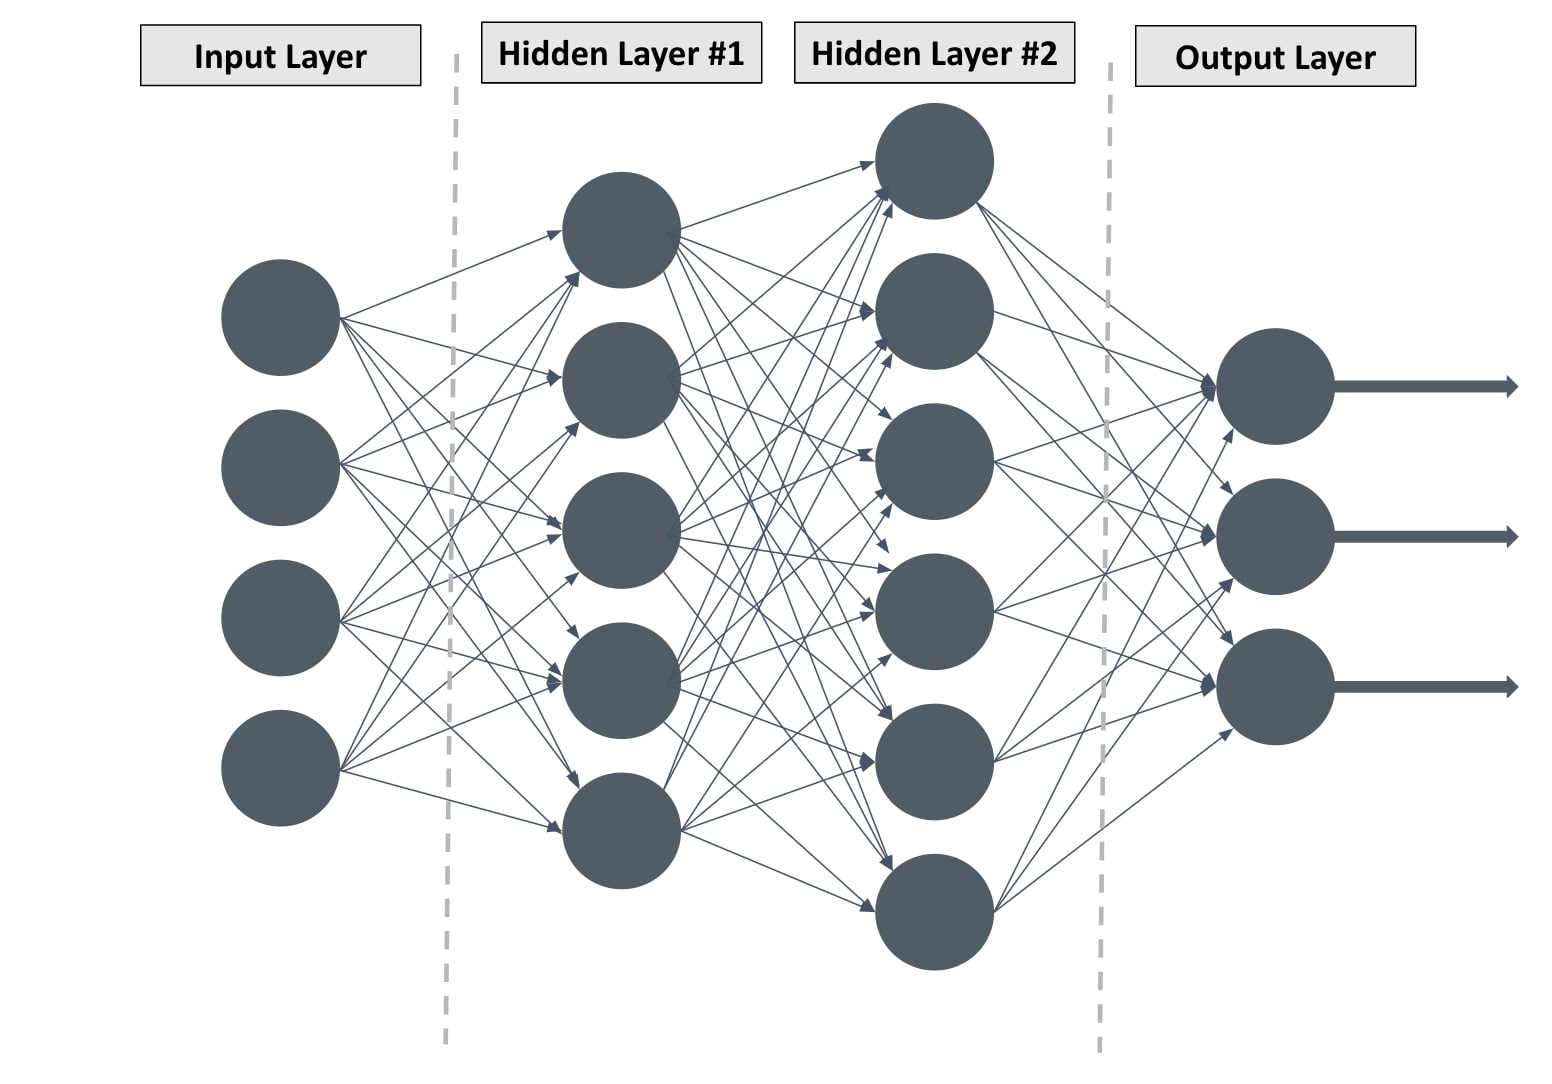
\includegraphics[width=0.7\textwidth]{../img/neoantigen/deep_nn}
	\caption{Representación de un \textit{Deep Feedforward Network}. Fuente: \cite{el2022machine}.}
	\label{fig:dnn}
\end{figure}


Por ejemplo una red neuronal como la presentada en la Figura \ref{fig:deep_nn}, se puede representar por la Ecuación \ref{equa:dl_1}. Donde se describe al vector de unidades ocultas en la capa $k$ como $\mathbf{h_k}$. El vector de \textit{bias} que contribuye a las capa oculta $k+1$ es $\mathbf{\beta_k}$. Los pesos que son aplicados a la $k^{th}$ capa y contribuyen a la capa $(k+1)^{th}$ es $\mathbf{\Omega_k}$. Entonces, una red neuronal profunda $y = f[x, \phi]$ con $k$ capas, se representa como:

\begin{equation}\label{equa:dl_1}
	\begin{gathered}
		\mathbf{h_1 = a [ \beta_{0} + \Omega_{0}x  ]}	 \\
		\mathbf{h_2 = a [ \beta_{1} + \Omega_{1} h_1  ]}	 \\
		\mathbf{h_3 = a [ \beta_{2} + \Omega_{2} h_2  ]}	 \\
		... \\
		\mathbf{h_k = a [ \beta_{k-1} + \Omega_{k-1} h_{k-1}  ]}	 \\
		\mathbf{y = \beta_{k} + \Omega_{k} h_{k} }	 \\
	\end{gathered}
\end{equation}

\begin{figure}[]
	\centering
	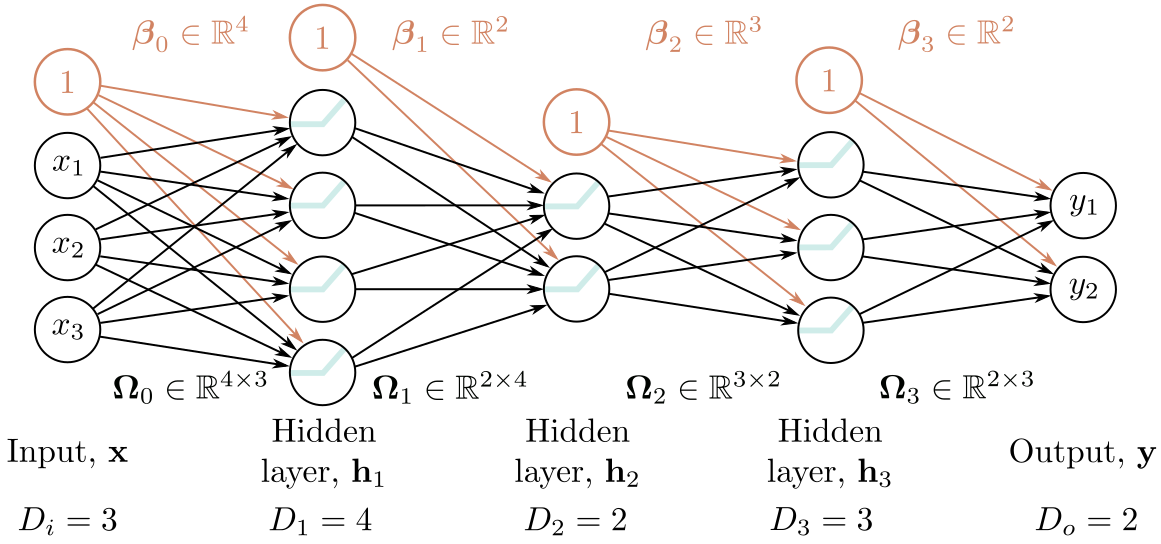
\includegraphics[width=0.78\textwidth]{../img/theory/deep_nn}
	\caption{Notación matricial de una red neuronal profunda. Fuente: \cite{prince2023understanding}.}
	\label{fig:deep_nn}
\end{figure}


\subsection{Redes Neuronales Convolucionales}

Una \textit{Convolutional Neural Networks} (CNN) o Red Neuronal Convolucional, es una red neuronal basada en la operación de convoluciones (utilizada en procesamiento de imágenes). Generalmente estas redes neuronales se aplican a problemas de visión computacional \citep{zhang2021dive}. Por ejemplo en la Figura \ref{fig:cnn_1d}, se presenta una red neuronal convolucional 1D con un \textit{kernel} de tamaño 3.  Cada salida $z_i$ es una suma ponderada de los tres inputs más cercanos $x_{i-1}, x_{i}, x_{i+1}$, donde los pesos son $[\omega_1, \omega_2, \omega_3]$. La salida $z_2$ se calcula con $z_2 = \omega_1x_1 + \omega_2x_2 + \omega_3x_3$. La salida $z_3 = \omega_1x_2 + \omega_2x_3 + \omega_3x_4$. Además, podemos variar el tamaño del \textit{kernel},  el \textit{stride} y \textit{dilation} como se ve en la Figura \ref{fig:conv1d}.

\begin{figure}[H]
	\centering
	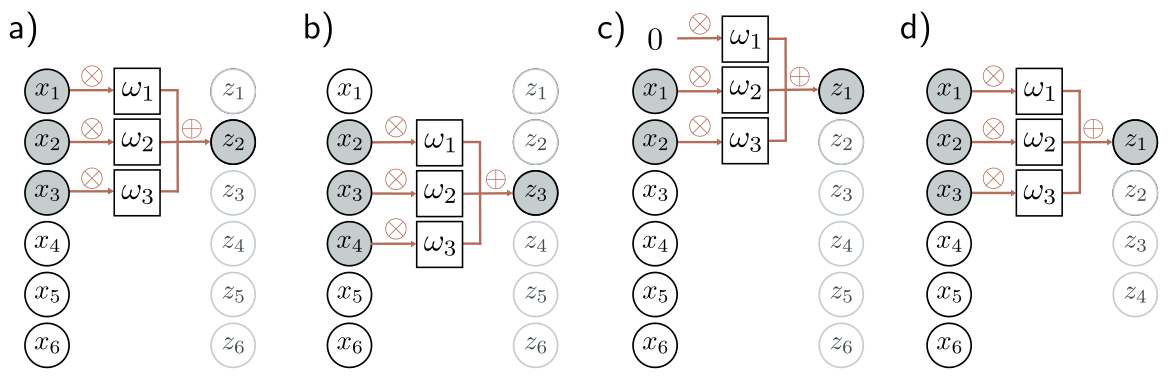
\includegraphics[width=\textwidth]{../img/theory/cnn}
	\caption{Red neuronal convolucional 1D con un \textit{kernel} de tamaño 3. Fuente: \cite{prince2023understanding}.}
	\label{fig:cnn_1d}
\end{figure}



\begin{figure}[H]
	\centering
	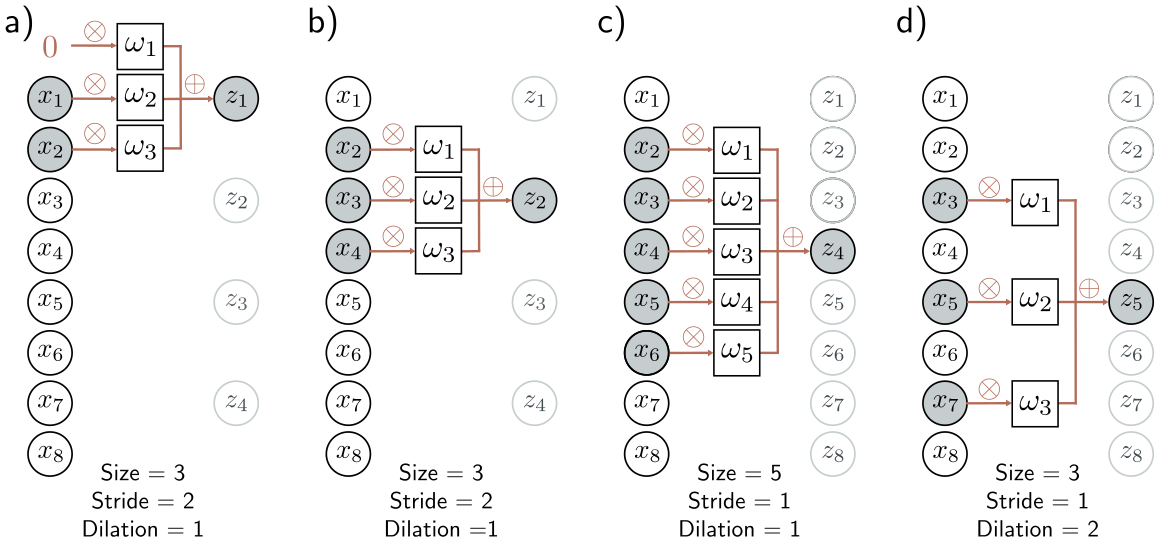
\includegraphics[width=\textwidth]{../img/theory/conv1d}
	\caption{Ejemplo del uso de \textit{stride, kernel size} y \textit{dilation} en la convolución 1D. Fuente: \cite{prince2023understanding}.}
	\label{fig:conv1d}
\end{figure}

Entonces, una capa convolucional calcula su salida convolucionando la entrada, sumando un \textit{bias} $\beta$, y pasando cada resultado a través de una función de activación $a[\bullet]$. Con un tamaño de \textit{kernel} de tres, \textit{stride} y \textit{dilation} igual a 1, la i-ésima unidad oculta $h_i$ se calcularía como:

\begin{equation}
	\begin{gathered}
	h_i = a [ \beta + \omega_1x_{i-1} + \omega_2x_{i} + \omega_3x_{i+1}] \\
	h_i = a \left[ \beta + \sum_{j=1}^{3} \omega_1x_{i-1} \right]
	\end{gathered}
\end{equation}


Adicionalmente, la operación básica es la convolución 2D, se presenta en la Figura \ref{fig:cnn}. Se toman pequeñas ventanas de una imagen y se realiza el producto punto con un \textit{kernel} ya establecido. Según los diferentes valores del \textit{kernel}, se pueden obtener diferentes resultados en la imagen de salida como: detección de bordes, suavizados, dilatación, etc. También puede ver la Figura \ref{fig:conv2d}, para ver el cómputo de una capa convolucional 2D.


\begin{figure}[H]
	\centering
	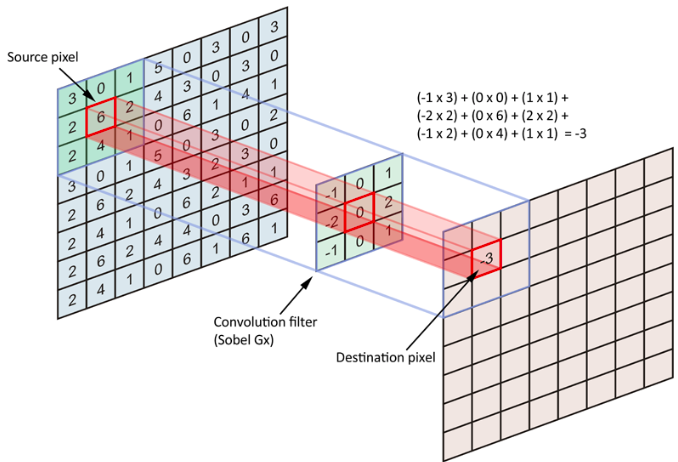
\includegraphics[width=0.7\textwidth]{../img/neoantigen/cnn}
	\caption{Ejemplo de una convolución 2D en procesamiento de imágenes. Fuente: \cite{Shuchen2022}.}
	\label{fig:cnn}
\end{figure}

\begin{figure}[h]
	\centering
	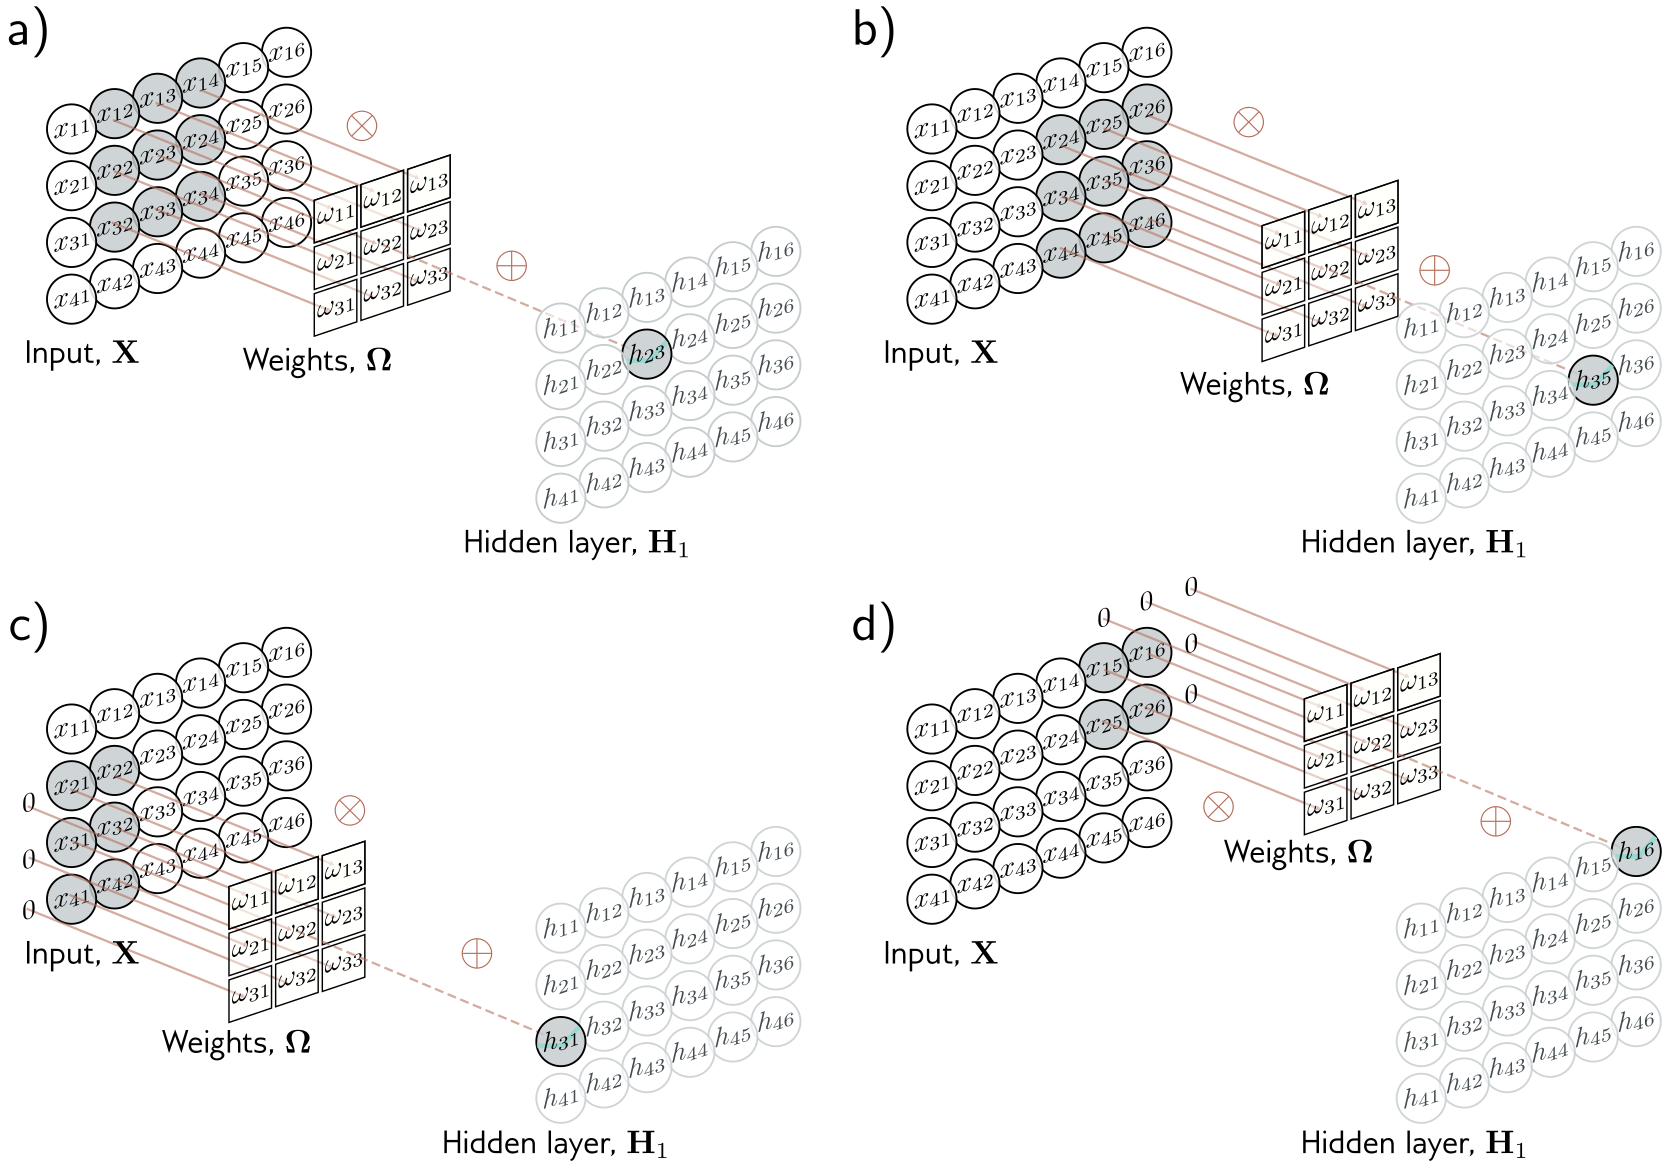
\includegraphics[width=\textwidth]{../img/theory/conv2d}
	\caption{Ejemplo de una capa convolucional 2D. Fuente: \cite{prince2023understanding}.}
	\label{fig:conv2d}
\end{figure}

Con inspiración en la operación de convolución, se plantean las CNN por primera vez por \cite{lecun1998gradient}. En la Figura \ref{fig:cnn3}, se presenta la LeNet-5, planteado por los autores. Luego, surgen diversa propuestas como AlexNet \citep{krizhevsky2012imagenet}, VGGNet \citep{simonyan2014very}, GoogleNet \citep{szegedy2015going} y ResNet \citep{he2016deep}.

\begin{figure}[H]
	\centering
	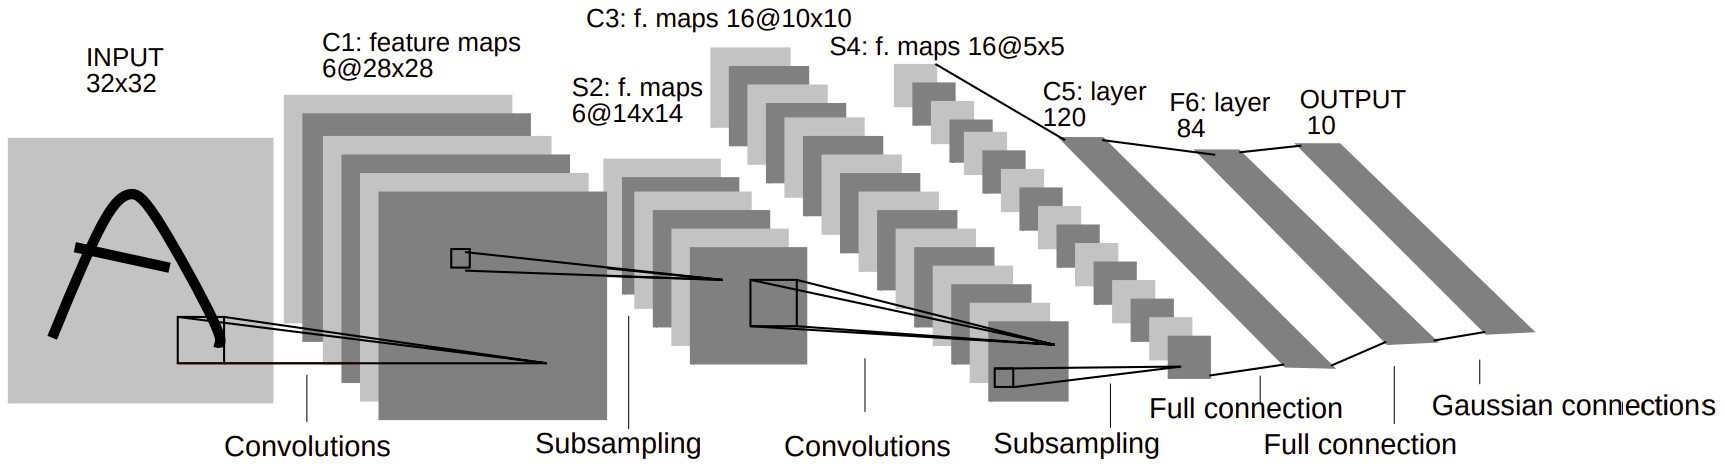
\includegraphics[width=\textwidth]{../img/neoantigen/cnn3}
	\caption{Arquitectura de LeNet-5, una CNN para el reconocimiento de dígitos. Fuente: \cite{lecun1998gradient}.}
	\label{fig:cnn3}
\end{figure}


\subsection{Redes Neuronales Recurrentes}

Mientras que las CNN están especializadas para manejar información espacial, las \textit{Recurrent Neural Networks} (RNN), se especializan en información secuencial  \citep{zhang2021dive}. En este campo, se habla del tiempo como una variable y se tratan problemas de series temporales por ejemplo.

El término RNN, aparece por primera vez en los trabajos de \cite{rumelhart1985learning} y \cite{jordan1997serial}. Algunos autores, comentan también que el inicio de las RNN fue con las redes de Hopfield  \citep{hopfield1982neural}. En general estas RNN, tienen dos entradas: estado actual y estado anterior; luego la RNN predice el siguiente estado. El problema de estas redes neuronales surgen por una falta de memoria, es decir cuando tenemos varios estados, el estado inicial va a influenciar cada vez menos a los estados futuros.

Como alternativa de solución al problema mencionado anteriormente, surge \textit{Long Short-Term Memory} (LSTM), propuesta por \cite{hochreiter1997long}. Una red neuronal LSTM, es capaz de recordar un dato relevante de una secuencia y almacenarlo varios instantes de tiempo. En la Figura \ref{fig:lstm}, explicamos brevemente el funcionamiento de LSTM, los datos que ingresan a una compuerta (\textit{gate}), son los datos de entrada en un tiempo específico y el estado oculto anterior. Luego, es procesado por tres capas totalmente conectadas: \textit{input gate}, \textit{forget gate} y \textit{output gate} \citep{zhang2021dive}.

\begin{figure}[H]
	\centering
	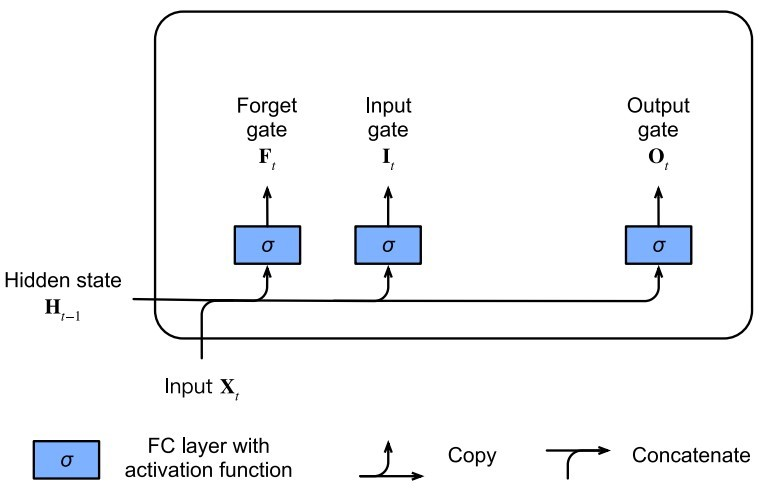
\includegraphics[width=0.7\textwidth]{../img/neoantigen/lstm}
	\caption{Ejemplo del procesamiento del \textit{input gate}, \textit{forget gate} y \textit{output gate} de LSTM. Fuente: \cite{zhang2021dive}.}
	\label{fig:lstm}
\end{figure}

\subsection{\textit{Transformers}}

%Los \textit{Transformers} son propuestas por \cite{vaswani2017attention}, para dar solución al problema de \textit{long-range dependency}. Por ejemplo el autor comenta: ``The Transformer is the first transduction model relying entirely on self-attention to compute representations of its input and output without using sequence-aligned RNNs or convolution''. Del enunciado anterior, \textit{transduction} hace referencia a la conversión secuencias de entrada hacia otro formato. Otro termino interesante es \textit{self-attention} (Figura \ref{fig:transformer}), este permite al modelo mirar hacia otras palabras en la secuencia de entrada para tener un mejor entendimiento de cierta palabra en la secuencia  \citep{Kelvin_transformer2022}.  

El concepto del mecanismo de atención fue introducido inicialmente por Bahdanau en 2014 \citep{bahdanau2014neural} para abordar las limitaciones asociadas con vectores de codificación de longitud fija. Este enfoque novedoso produjo resultados comparables a los estados del arte en la traducción de inglés a francés. Posteriormente, el mecanismo de atención encontró aplicación en la inferencia de lenguaje natural \citep{parikh2016decomposable}, lo que llevó a la propuesta de una red de atención estructurada \citep{kim2017structured}. Sin embargo, es importante señalar que estos módulos de atención se utilizaban típicamente en conjunto con redes recurrentes. Ocurrió un cambio significativo en 2017 con la publicación del innovador artículo \textit{``Attention Is All You Need''} propuesta por \cite{vaswani2017attention}, que presentó una nueva arquitectura de red conocida como \textit{Transformer}. Esta arquitectura se basó exclusivamente en mecanismos de atención y representó una partida fundamental de los enfoques tradicionales. En 2018, \cite{devlin2018bert} introdujo el modelo bidireccional de \textit{Transformer Bidirectional Encoder Representations from Transformers} (BERT). Desde entonces, se ha convertido en uno de los modelos de \textit{Transformer} más reconocidos e influyentes en el campo. El \textit{Transformer} se basa en el concepto de \textit{self-attention}, que se refiere a cuánta atención presta una palabra a otras palabras. Por ejemplo, en la siguiente oración: ``El animal no cruzó la calle porque estaba muy cansado'', \textit{self-attention} permite asociar ``estaba'' con ``animal'' \citep{prince2023understanding}.

\subsubsection{\textit{Self-attention}}

El bloque principal de un \textit{Transformer}, es la autoatención o \textit{self-attention} $sa[\bullet]$, que toma $N$ entradas $x_n$, cada una de dimensión $D \times 1$, y devuelve $N$ vectores de salida del mismo tamaño. En el procesamiento del lenguaje natural, cada entrada $x_n$ representa una palabra; mientras que en secuencias de proteínas, representa un aminoácido. Luego, por cada entrada, se calcula un conjunto de valores $v_m = \beta_v + \Omega_vx_m$, donde $\beta_v$ y $\Omega_v$ son los sesgos y pesos, respectivamente. Así, el bloque de \textit{self-attention} se calcula mediante la Ecuación \ref{eq:self-attention}. Además, $a[x_m, x_m]$ es la atención que la salida $x_n$ presta a $x_m$ y se calcula mediante el producto punto entre $k_m^T$ y $q_n$. Adicionalmente, se prefiere trabajar con un \textit{self-attention}  escalado (Ecuación \ref{eq:scaled-self-attention}); aquí, $D_q$ es la dimensión de $q_n$ y $k_n$. En la Figura \ref{fig:t_1}, se ejemplifica el proceso para calcular \textit{self-attention}, mientras que en la Figura \ref{fig:self-attention}, se presenta lo mismo, pero forma matricial \citep{prince2023understanding}.


\begin{equation}\label{eq:attention}
	\begin{gathered}
	v_m = \beta_v + \Omega_vx_m \\
	q_n = \beta_q + \Omega_qx_n \\
	k_n = \beta_k + \Omega_kx_m \\
	a[x_m, x_n] = \mbox{softmax}[k_m^T \cdot q_n]
	\end{gathered}
\end{equation}

\begin{equation}\label{eq:self-attention}
	Sa[X] = V \cdot \mbox{softmax}[ k^T \cdot q_n ]   
\end{equation}

\begin{equation}\label{eq:scaled-self-attention}
	\mbox{Sa}[X] = V \cdot \mbox{softmax}\left[ \frac{k^T \cdot q_n}{ \sqrt{D_q} }   \right]   
\end{equation}


\begin{figure}
	\centering
	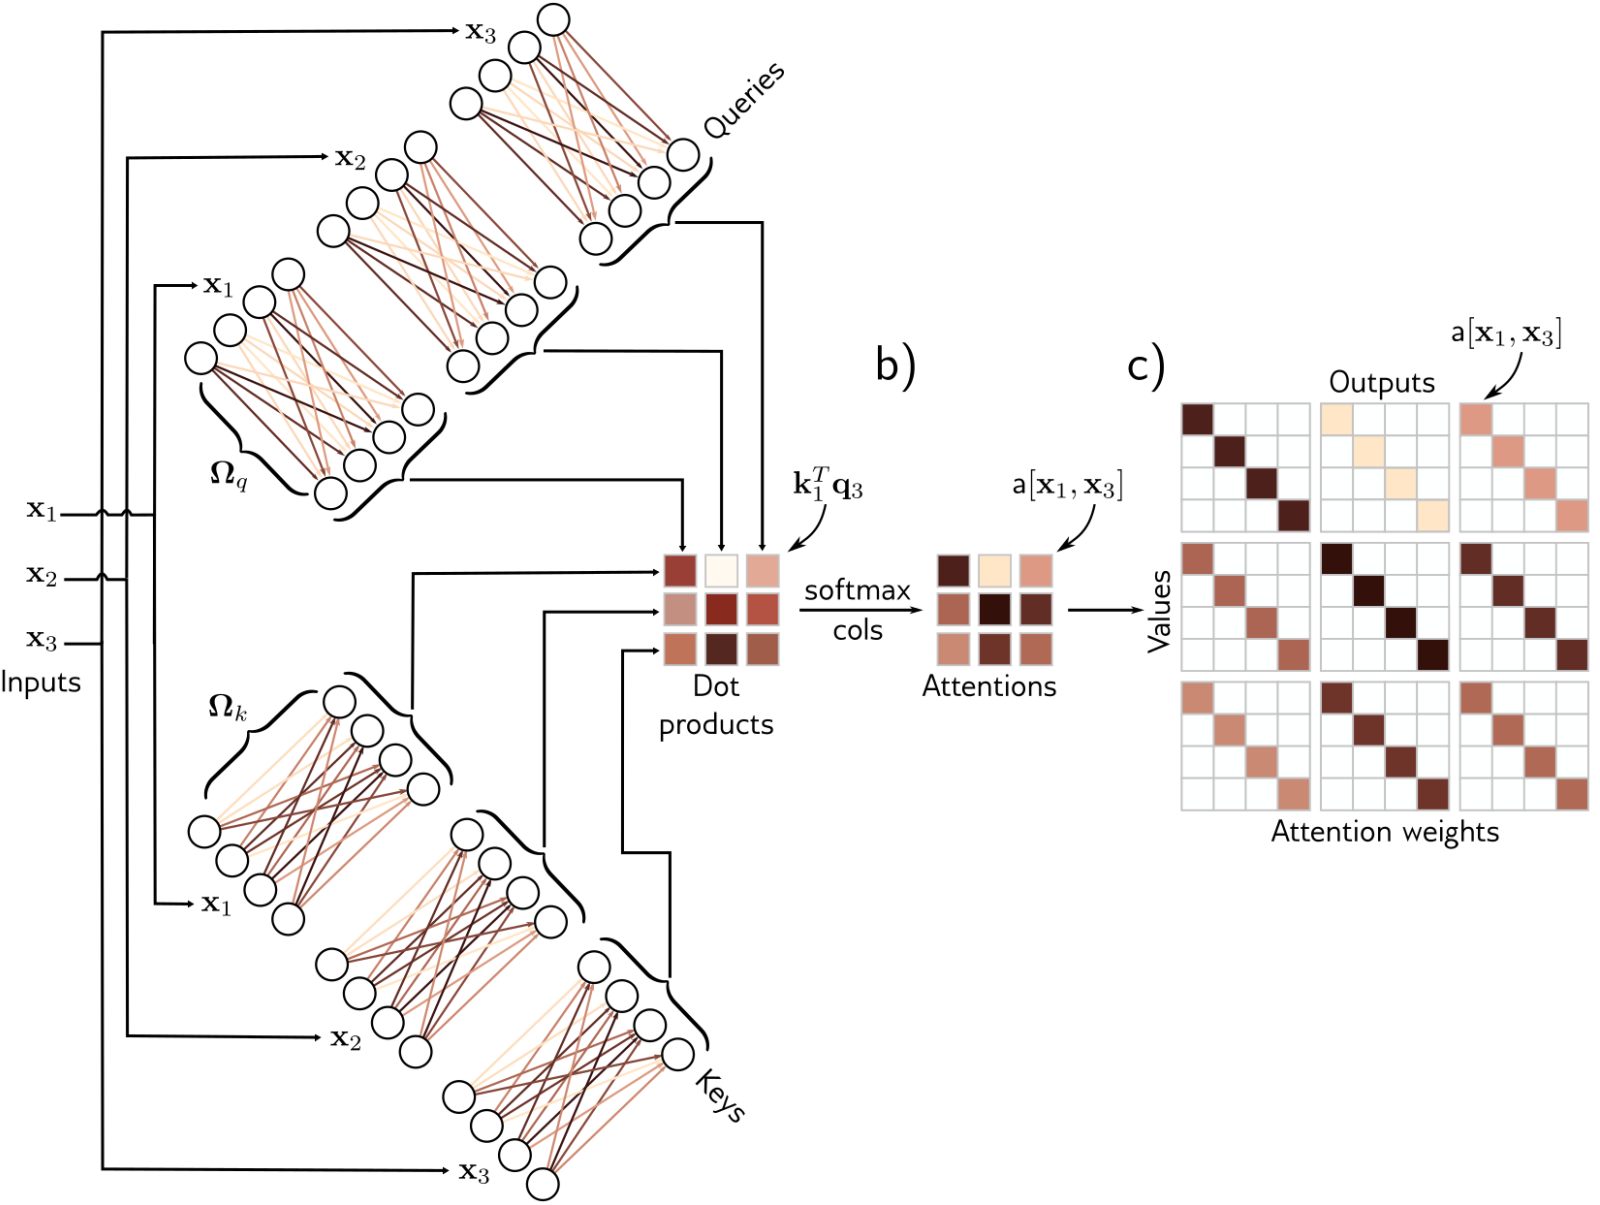
\includegraphics[width=\textwidth]{../img/theory/t_1}
	\caption{Ejemplo de como calcular \textit{self-attention}. Fuente: \cite{prince2023understanding}}
	\label{fig:t_1}
\end{figure}

Además, aplicar varios \textit{multi-head self-attention} logra mejores resultados \citep{prince2023understanding}. Entonces, la concatenación de varios \textit{head attentions} se presenta en la Ecuación \ref{multihead}.

\begin{equation}\label{multihead}
	\mbox{MhSa}[X] = \Omega_c[Sa_1[X]; Sa_2[X];...;Sa_H[X];]
\end{equation}

\begin{figure}
	\centering
	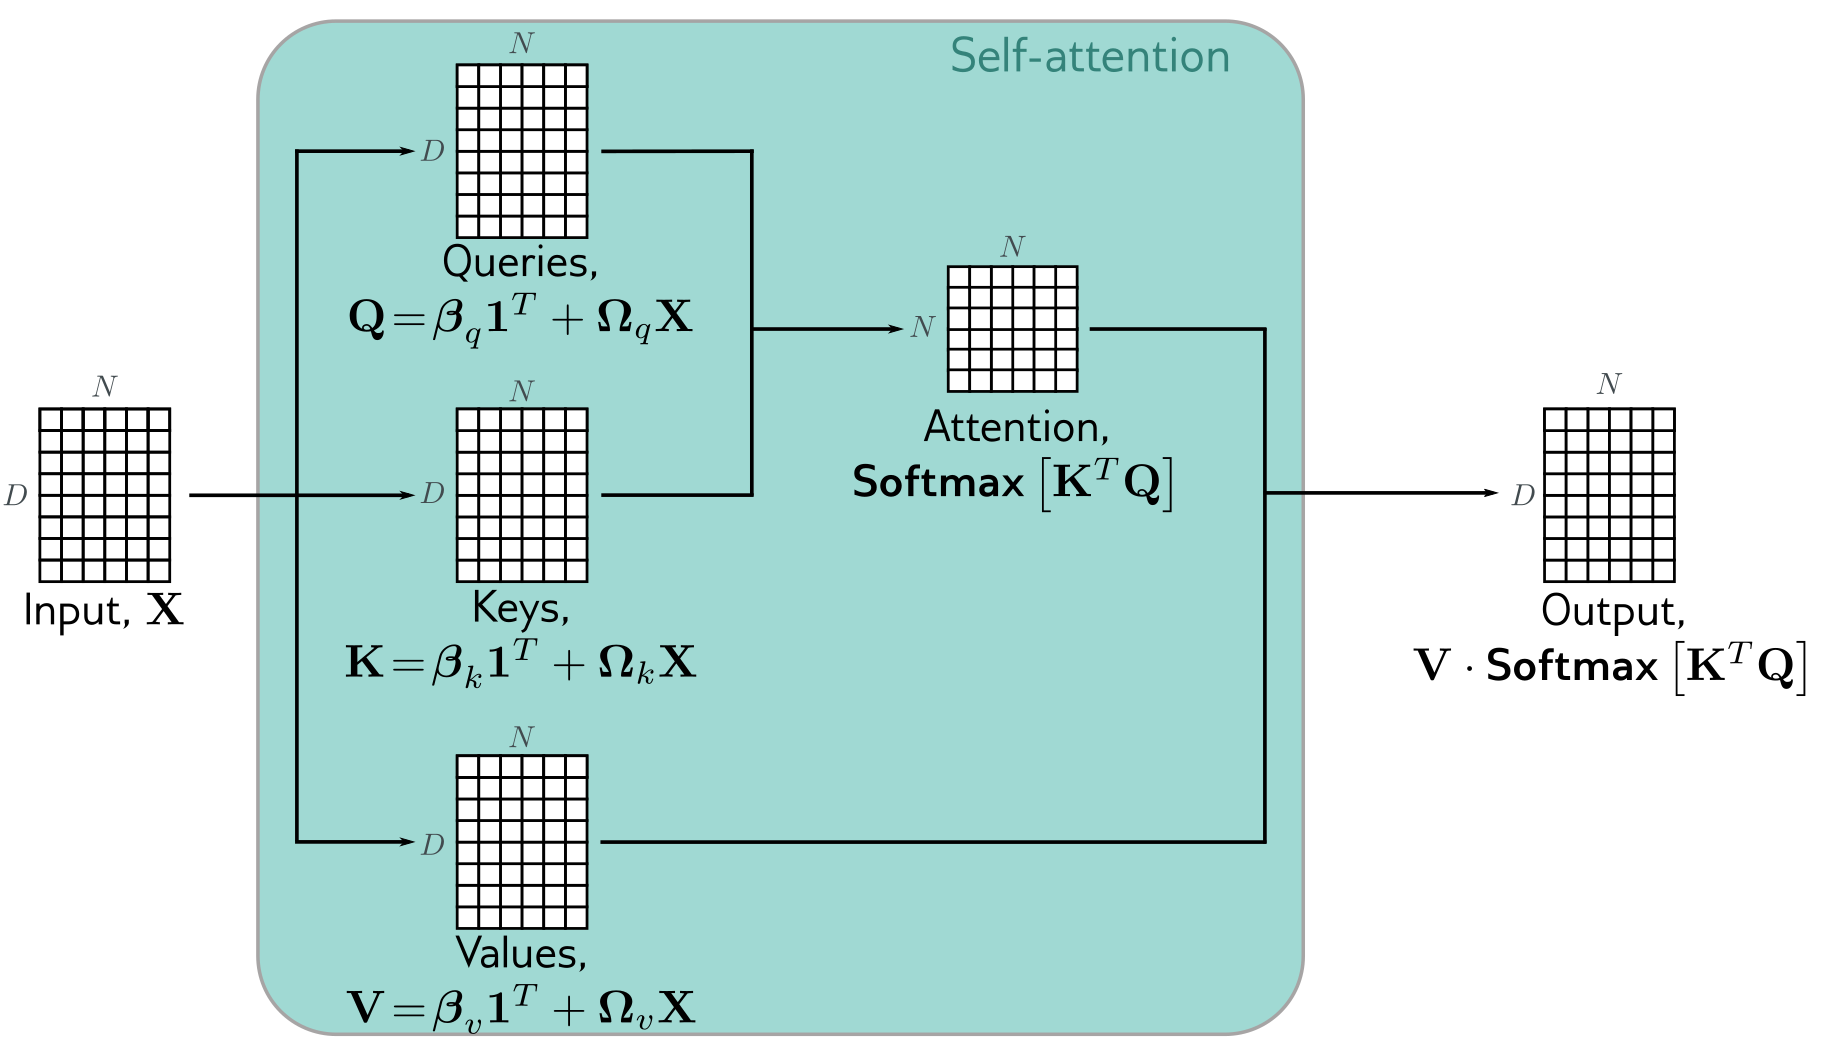
\includegraphics[width=0.9\textwidth]{../img/theory/attention_weights_matrix.png}
	\caption{Proceso para procesar el \textit{self-attention} de forma matricial. Fuente: \cite{prince2023understanding}}
	\label{fig:self-attention}
\end{figure}

%\begin{figure}[H]
%	\centering
%	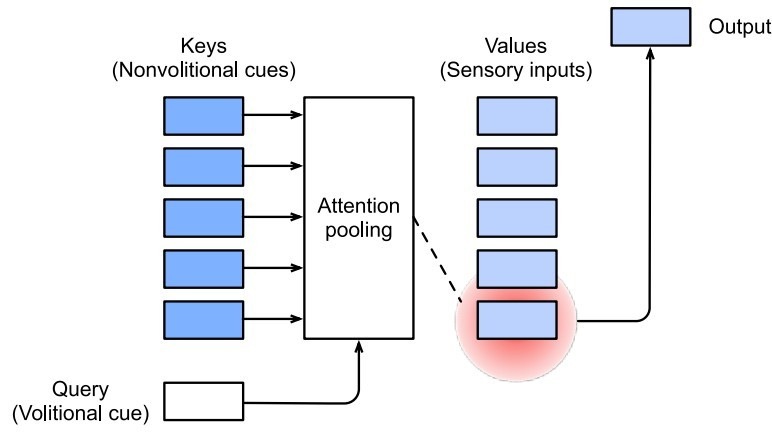
\includegraphics[width=0.7\textwidth]{img/neoantigen/transformer}
%	\caption{Ejemplo del mecanismo de atención de una red \textit{Transformer}. Fuente: \cite{zhang2021dive}.}
%	\label{fig:transformer}
%\end{figure}


\subsubsection{\textit{Mulitple head self-attention}}

Normalmente se aplican múltiples mecanismos de \textit{self-attention} en paralelo, y esto se conoce como \textit{multiple head self-attention}. Ahora se calculan $H$ conjuntos diferentes de $v$, $k$ y $q$ \citep{prince2023understanding}:

\begin{equation}\label{eq:mha}
	\begin{gathered}
		\mathbf{ V_m = \beta_{vh}1^T + \Omega_{vh}X }\\
		\mathbf{Q_n = \beta_{qh}1^T + \Omega_{qh}X }\\
		\mathbf{K_n = \beta_{kh}1^T + \Omega_{kh}X }	
	\end{gathered}
\end{equation}

El $h^{th}$ \textit{self-attention} se calcula con:

\begin{equation}\label{eq:mha2}	
\mathbf{Sa_h[X] = V_h \cdot \mbox{Softmax}\left[ \frac{K_h^T Q_h}{ \sqrt{D_q} }  \right]}	
\end{equation}

Un resumen, es presentado en la Figura \ref{fig:mhsa}.

\begin{figure}
	\centering
	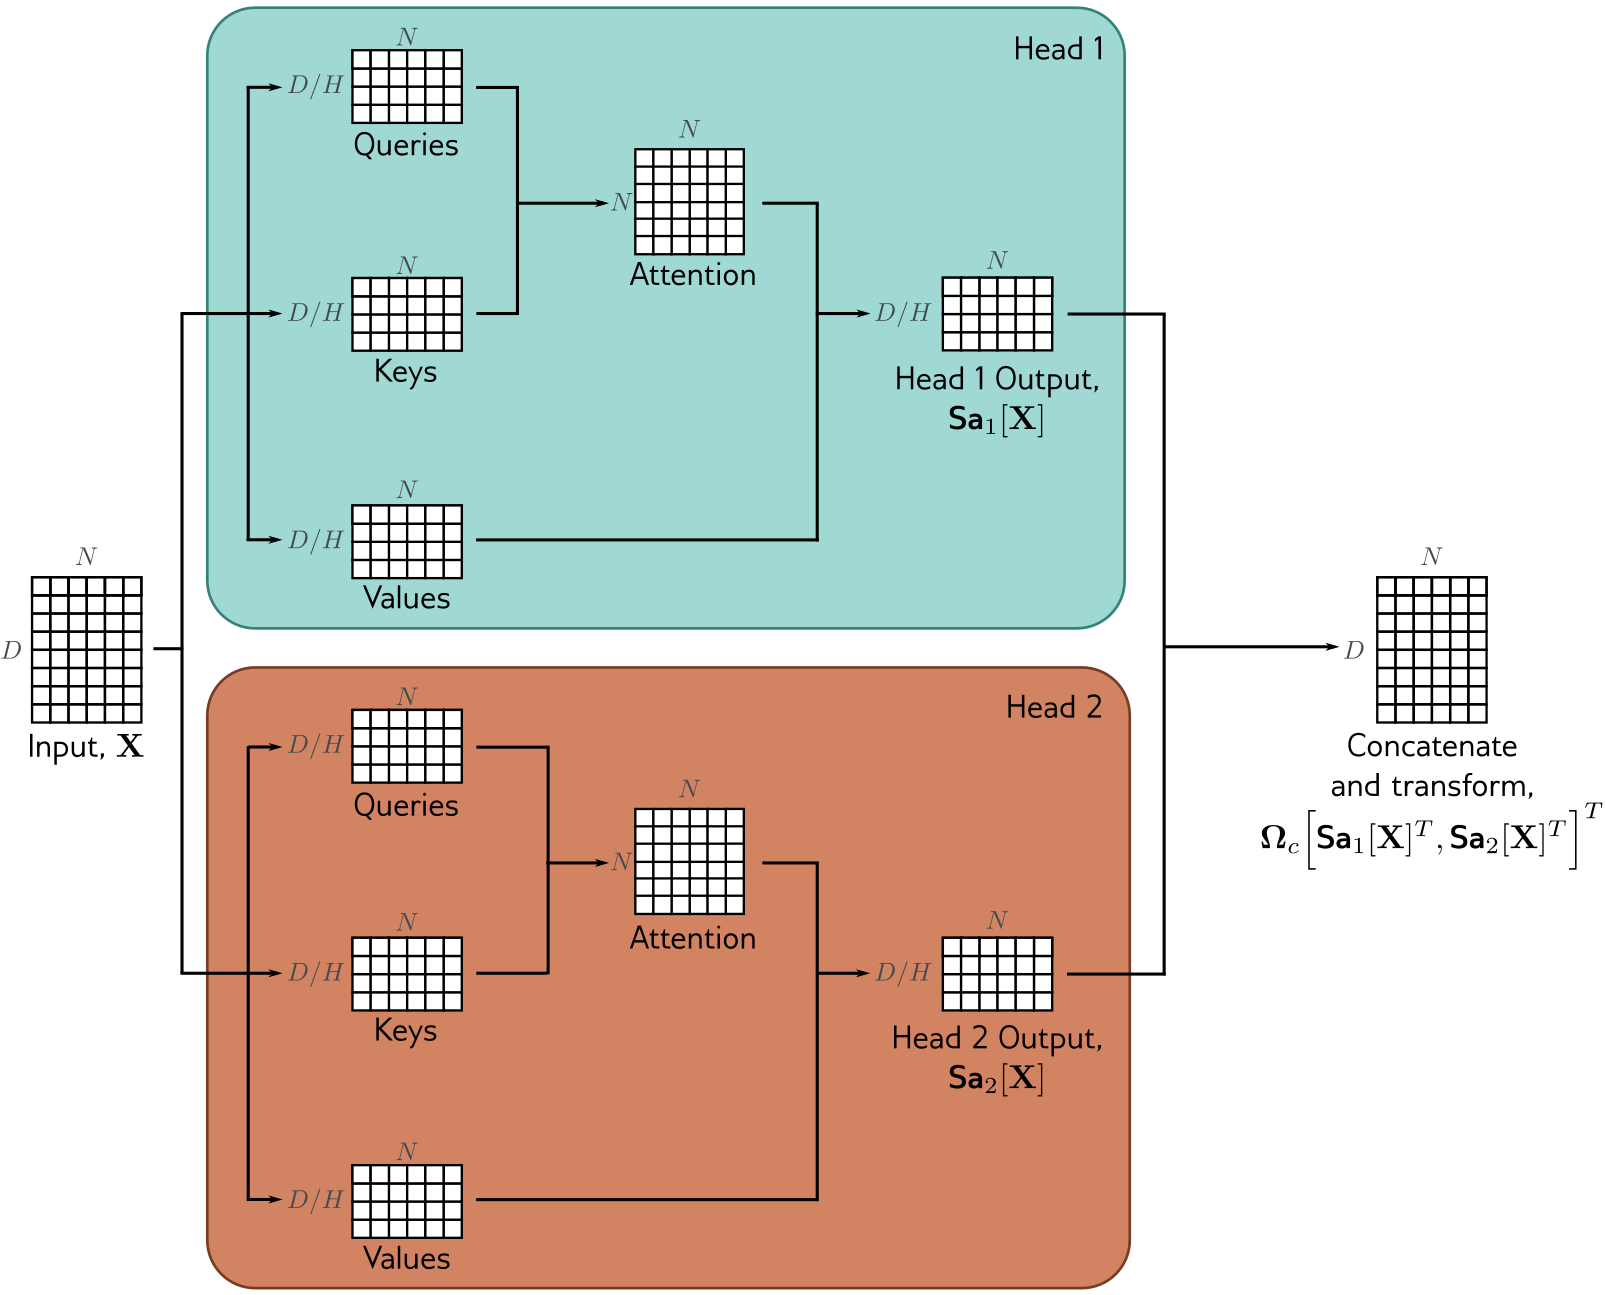
\includegraphics[width=\textwidth]{../img/theory/mhsa}
	\caption{Proceso para procesar el \textit{multiple head self-attention}. Fuente: \cite{prince2023understanding}}
	\label{fig:mhsa}
\end{figure}


\subsection{BERT}

\textit{Bidirectional Encoder Representations from Transformers} (BERT), propuesta por \cite{devlin2018bert}, está inspirada por la red \textit{Transformer} y su mecanismo de atención, la cuál entiende la relación contextual entre diferentes palabras. A diferencia de una RNN, BERT no tiene dirección, es decir lee la secuencia entera. Esta característica, le permite al modelo aprender información contextual de una palabra con respecto a las otras \citep{Kelvin_transformer2022}.


BERT es un modelo de codificador que utiliza un vocabulario de 30000 \textit{tokens}. Los \textit{tokens} de entrada se convierten en \textit{word-embedding} de dimensión 1024 y se pasan a través de 24 \textit{Transformers}. Cada uno de ellos contiene un mecanismo de \textit{self-attention} con 16 \textit{heads}. Los \textit{queries, keys} y \textit{values} para cada \textit{head} tienen una dimensión de 64. La dimensión de la única capa oculta en la red completamente conectada en el \textit{Transformer} es de 4096. El número total de parámetros es aproximadamente 340 millones. Cuando se introdujo BERT, esto se consideraba grande, pero ahora es mucho más pequeño que los modelos de vanguardia \citep{prince2023understanding}.

\subsubsection{Pre-entrenamiento}

En la etapa de pre-entrenamiento, la red se entrena utilizando \textit{self-supervision}. Esto permite el uso de cantidades enormes de datos sin necesidad de etiquetas manuales. En el caso de BERT, la tarea de \textit{self-supervision} consiste en predecir las palabras faltantes en oraciones tomadas de un gran corpus de internet (Figura \ref{fig:bert}). Durante el entrenamiento, la longitud máxima de entrada es de 512 \textit{tokens} y el tamaño del \textit{batch size} es de 256. El sistema se entrena durante un millón de \textit{steps}, lo que equivale aproximadamente a 50 \textit{epochs} del corpus de 3.3 mil millones de palabras \citep{prince2023understanding}.

\begin{figure}[H]
	\centering
	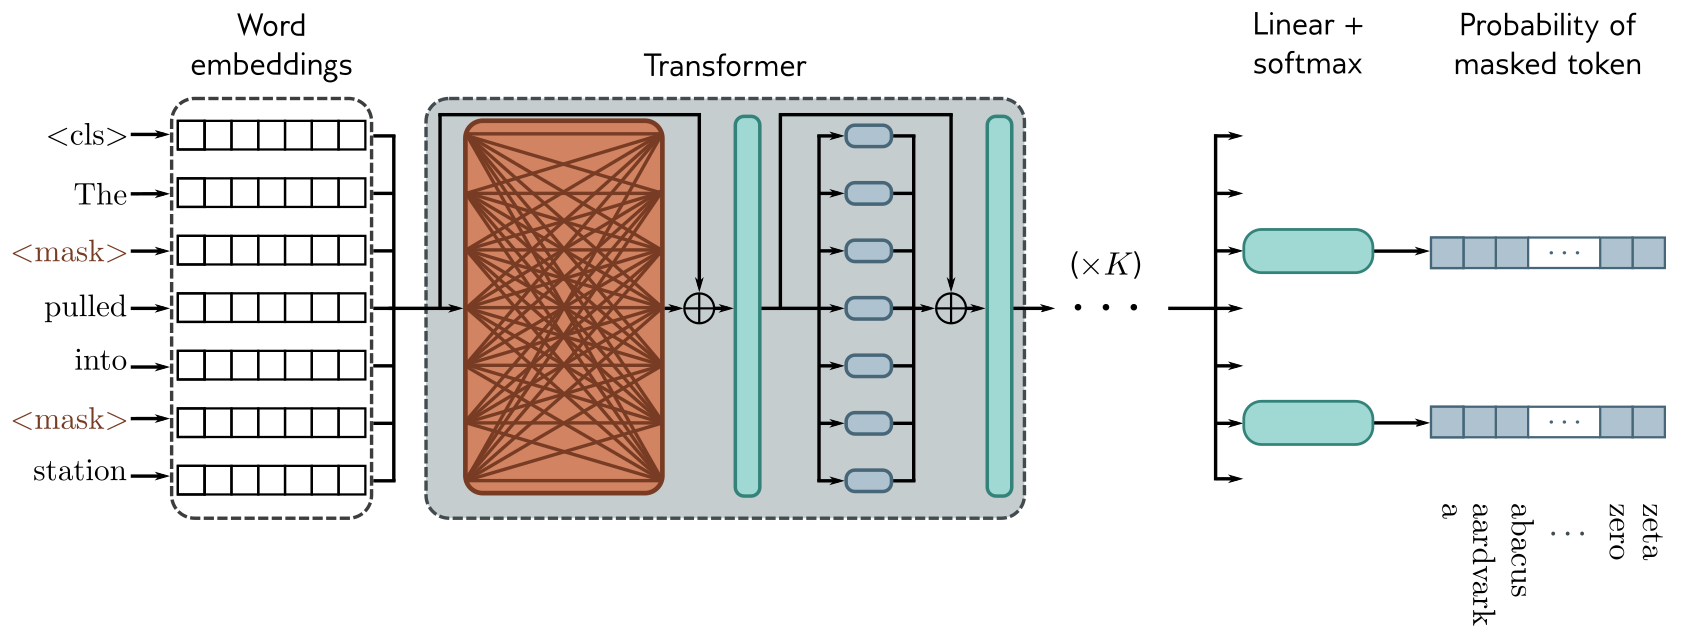
\includegraphics[width=\textwidth]{../img/theory/pre-training}
	\caption{Pre-entrenamiento de BERT. Fuente: \cite{prince2023understanding}}
	\label{fig:bert}
\end{figure}


\subsubsection{\textit{Fine-tuning}}



En la etapa de \textit{fine-tuning}, los parámetros del modelo se ajustan para especializar la red en una tarea particular. Se añade una capa adicional a la red del \textit{Transformer} para convertir los vectores de salida al formato de salida deseado \citep{prince2023understanding}. Por ejemplo, se puede realizar  para la tarea de clasificación de textos (Figura \ref{fig:bert2}.a); donde, se coloca un token especial conocido como el token de clasificación o \textit{cls} al comienzo de cada cadena durante el pre-entrenamiento. Para tareas de clasificación de texto como el análisis de sentimientos (en el cual el pasaje se etiqueta como tener un tono emocional positivo o negativo), el vector asociado con el token \textit{cls} se asigna a un número único y se pasa a través de una función sigmoidea \citep{prince2023understanding}.

También, se puede realizar nuevas tareas como clasificación de palabras. El objetivo es clasificar cada palabra como un tipo de entidad (por ejemplo, persona, lugar, organización o ninguna entidad), como se describe en la Figura \ref{fig:bert2}.b \citep{prince2023understanding}.

\begin{figure}[H]
	\centering
	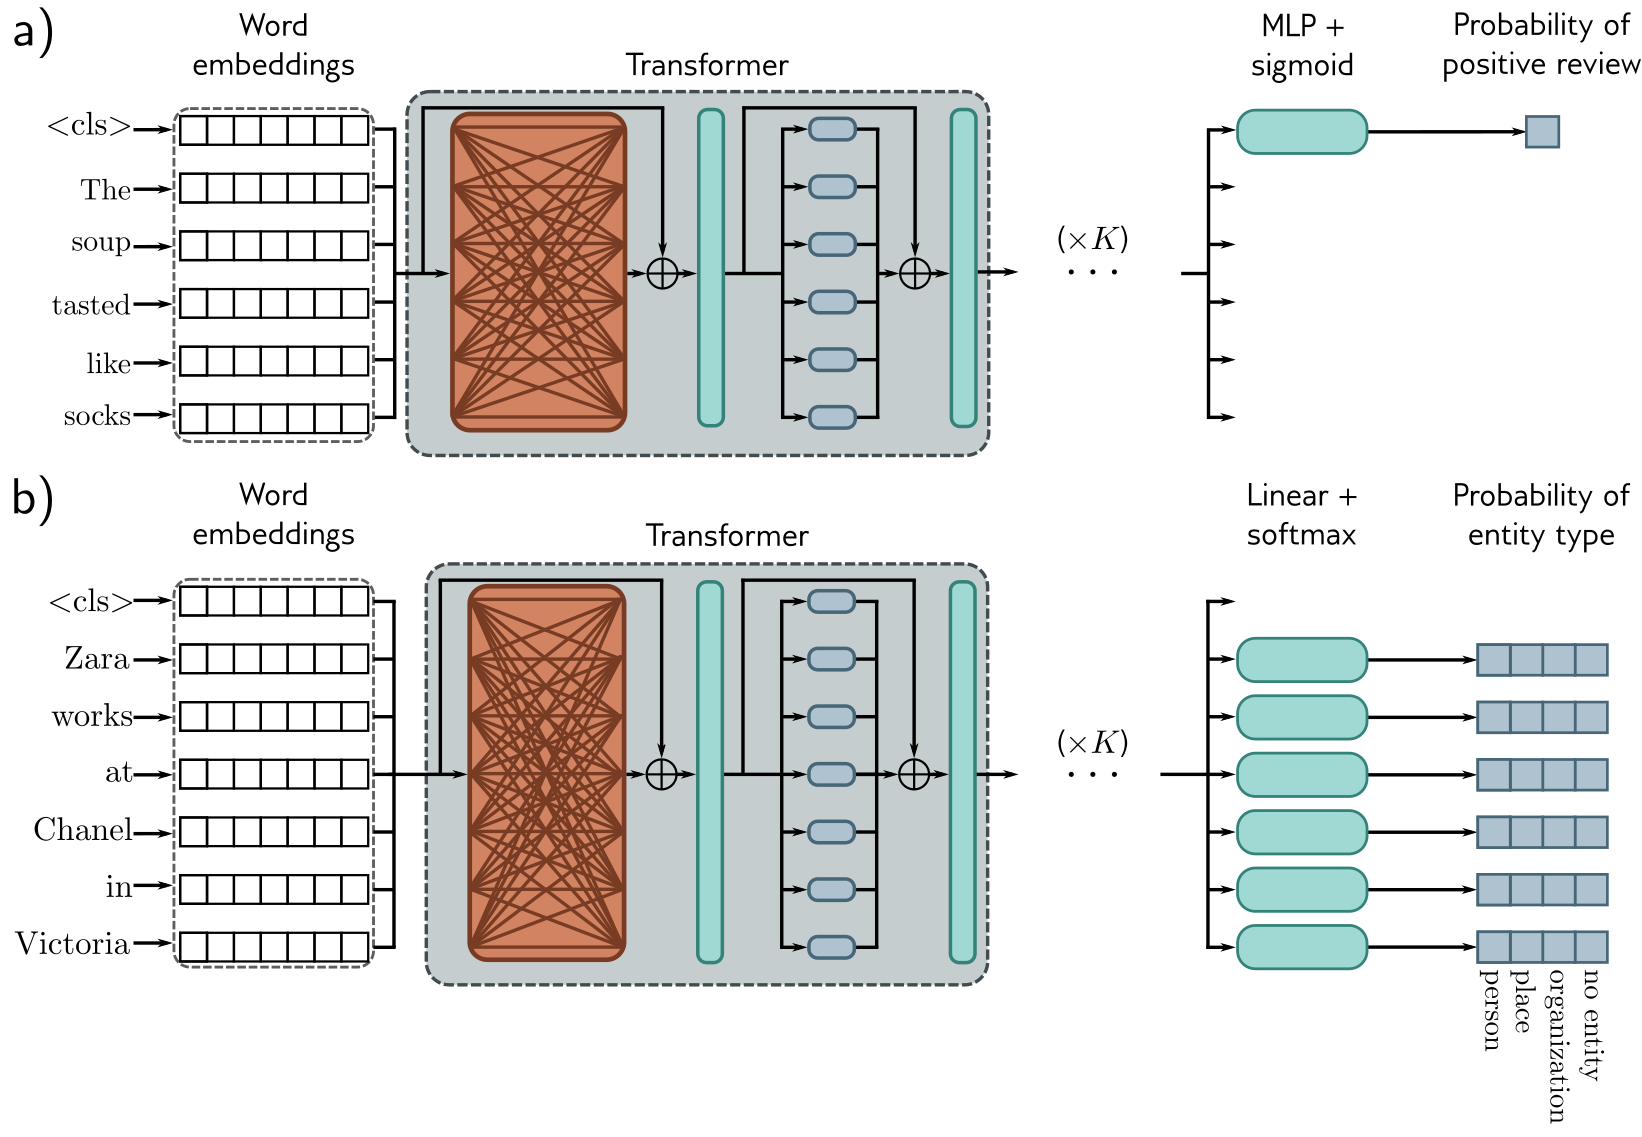
\includegraphics[width=\textwidth]{../img/theory/pre-training2}
	\caption[\textit{Fine-tuning} de BERT]{\textit{Fine-tuning} de BERT, luego del pre-entrenamiento se realiza \textit{fine-tuning} sobre un conjunto de datos etiquetados manualmente para una tarea específica. Fuente: \cite{prince2023understanding}}
	\label{fig:bert2}
\end{figure}


El \textit{fine-tuning} de modelos pre-entrenados mediante \textit{self-supervision} ha mejorado significativamente el rendimiento de vanguardia en tareas de procesamiento del lenguaje natural \citep{zhang2020revisiting}. Sin embargo, a pesar de los éxitos significativos, el \textit{fine-tuning} sigue siendo inestable, especialmente cuando se utiliza la variante grande de BERT en conjuntos de datos pequeños, donde el pre-entrenamiento tiene el potencial de proporcionar el beneficio más significativo. Procesos de aprendizaje idénticos con diferentes \textit{seeds} aleatorios a menudo resultan en modelos significativamente diferentes y a veces degenerados después del \textit{fine-tuning}, incluso cuando solo algunos aspectos aparentemente insignificantes del proceso de aprendizaje se ven afectados por el \textit{seed} aleatorio  \citep{zhang2020revisiting,prince2023understanding}.


\section{Conclusiones del marco conceptual}

En este capítulo hemos descrito los conceptos necesarios para comprender y analizar esta tesis. De esta forma hemos partido desde conocimientos básicos de biología molecular e inteligencia artificial. Se abarcó estos temas porque la propuesta de este proyecto se encuentra en la intersección de estas dos áreas.

La biología molecular  tiene un papel muy importante en la actualidad y además tiene muchos problemas aún por resolver. Aún no hemos entendido con precisión todo el genoma humano, así mismo, nuestro cuerpo esta compuesto por aproximadamente 10000 proteínas, pero aún no las conocemos todas, o no tenemos claro su papel biológico. Es mas, no conocemos su estructura y función. Y esto se complica mas, porque estas proteínas forman redes biológicas que determinan su función variable en el tiempo. Frente a este conjunto de problemas, han surgido métodos computacionales que buscan descubrir y entender la genómica, transcriptómica y proteómica; y ahora con la revolución de la inteligencia artificial y modelos Transformers, se ha empezado a descubrir nuevos métodos, soluciones a problemas que se consideraban imposibles de resolver, como por ejemplo la predicción de estructura de proteínas. Sin duda alguna, el uso de la inteligencia artificial, puede abrir muchas aplicaciones en la Bioinformática, ayudando a descubrir nuevos medicamentos, función de las proteínas, desarrollo de la medicina personalizada, etc.


%EOF
